\documentclass{article}
\usepackage{iclr2027_conference,times}
%%%%% NEW MATH DEFINITIONS %%%%%

\usepackage{amsmath,amsfonts,bm}

% Mark sections of captions for referring to divisions of figures
\newcommand{\figleft}{{\em (Left)}}
\newcommand{\figcenter}{{\em (Center)}}
\newcommand{\figright}{{\em (Right)}}
\newcommand{\figtop}{{\em (Top)}}
\newcommand{\figbottom}{{\em (Bottom)}}
\newcommand{\captiona}{{\em (a)}}
\newcommand{\captionb}{{\em (b)}}
\newcommand{\captionc}{{\em (c)}}
\newcommand{\captiond}{{\em (d)}}

% Highlight a newly defined term
\newcommand{\newterm}[1]{{\bf #1}}


% Figure reference, lower-case.
\def\figref#1{figure~\ref{#1}}
% Figure reference, capital. For start of sentence
\def\Figref#1{Figure~\ref{#1}}
\def\twofigref#1#2{figures \ref{#1} and \ref{#2}}
\def\quadfigref#1#2#3#4{figures \ref{#1}, \ref{#2}, \ref{#3} and \ref{#4}}
% Section reference, lower-case.
\def\secref#1{section~\ref{#1}}
% Section reference, capital.
\def\Secref#1{Section~\ref{#1}}
% Reference to two sections.
\def\twosecrefs#1#2{sections \ref{#1} and \ref{#2}}
% Reference to three sections.
\def\secrefs#1#2#3{sections \ref{#1}, \ref{#2} and \ref{#3}}
% Reference to an equation, lower-case.
\def\eqref#1{equation~\ref{#1}}
% Reference to an equation, upper case
\def\Eqref#1{Equation~\ref{#1}}
% A raw reference to an equation---avoid using if possible
\def\plaineqref#1{\ref{#1}}
% Reference to a chapter, lower-case.
\def\chapref#1{chapter~\ref{#1}}
% Reference to an equation, upper case.
\def\Chapref#1{Chapter~\ref{#1}}
% Reference to a range of chapters
\def\rangechapref#1#2{chapters\ref{#1}--\ref{#2}}
% Reference to an algorithm, lower-case.
\def\algref#1{algorithm~\ref{#1}}
% Reference to an algorithm, upper case.
\def\Algref#1{Algorithm~\ref{#1}}
\def\twoalgref#1#2{algorithms \ref{#1} and \ref{#2}}
\def\Twoalgref#1#2{Algorithms \ref{#1} and \ref{#2}}
% Reference to a part, lower case
\def\partref#1{part~\ref{#1}}
% Reference to a part, upper case
\def\Partref#1{Part~\ref{#1}}
\def\twopartref#1#2{parts \ref{#1} and \ref{#2}}

\def\ceil#1{\lceil #1 \rceil}
\def\floor#1{\lfloor #1 \rfloor}
\def\1{\bm{1}}
\newcommand{\train}{\mathcal{D}}
\newcommand{\valid}{\mathcal{D_{\mathrm{valid}}}}
\newcommand{\test}{\mathcal{D_{\mathrm{test}}}}

\def\eps{{\epsilon}}


% Random variables
\def\reta{{\textnormal{$\eta$}}}
\def\ra{{\textnormal{a}}}
\def\rb{{\textnormal{b}}}
\def\rc{{\textnormal{c}}}
\def\rd{{\textnormal{d}}}
\def\re{{\textnormal{e}}}
\def\rf{{\textnormal{f}}}
\def\rg{{\textnormal{g}}}
\def\rh{{\textnormal{h}}}
\def\ri{{\textnormal{i}}}
\def\rj{{\textnormal{j}}}
\def\rk{{\textnormal{k}}}
\def\rl{{\textnormal{l}}}
% rm is already a command, just don't name any random variables m
\def\rn{{\textnormal{n}}}
\def\ro{{\textnormal{o}}}
\def\rp{{\textnormal{p}}}
\def\rq{{\textnormal{q}}}
\def\rr{{\textnormal{r}}}
\def\rs{{\textnormal{s}}}
\def\rt{{\textnormal{t}}}
\def\ru{{\textnormal{u}}}
\def\rv{{\textnormal{v}}}
\def\rw{{\textnormal{w}}}
\def\rx{{\textnormal{x}}}
\def\ry{{\textnormal{y}}}
\def\rz{{\textnormal{z}}}

% Random vectors
\def\rvepsilon{{\mathbf{\epsilon}}}
\def\rvtheta{{\mathbf{\theta}}}
\def\rva{{\mathbf{a}}}
\def\rvb{{\mathbf{b}}}
\def\rvc{{\mathbf{c}}}
\def\rvd{{\mathbf{d}}}
\def\rve{{\mathbf{e}}}
\def\rvf{{\mathbf{f}}}
\def\rvg{{\mathbf{g}}}
\def\rvh{{\mathbf{h}}}
\def\rvu{{\mathbf{i}}}
\def\rvj{{\mathbf{j}}}
\def\rvk{{\mathbf{k}}}
\def\rvl{{\mathbf{l}}}
\def\rvm{{\mathbf{m}}}
\def\rvn{{\mathbf{n}}}
\def\rvo{{\mathbf{o}}}
\def\rvp{{\mathbf{p}}}
\def\rvq{{\mathbf{q}}}
\def\rvr{{\mathbf{r}}}
\def\rvs{{\mathbf{s}}}
\def\rvt{{\mathbf{t}}}
\def\rvu{{\mathbf{u}}}
\def\rvv{{\mathbf{v}}}
\def\rvw{{\mathbf{w}}}
\def\rvx{{\mathbf{x}}}
\def\rvy{{\mathbf{y}}}
\def\rvz{{\mathbf{z}}}

% Elements of random vectors
\def\erva{{\textnormal{a}}}
\def\ervb{{\textnormal{b}}}
\def\ervc{{\textnormal{c}}}
\def\ervd{{\textnormal{d}}}
\def\erve{{\textnormal{e}}}
\def\ervf{{\textnormal{f}}}
\def\ervg{{\textnormal{g}}}
\def\ervh{{\textnormal{h}}}
\def\ervi{{\textnormal{i}}}
\def\ervj{{\textnormal{j}}}
\def\ervk{{\textnormal{k}}}
\def\ervl{{\textnormal{l}}}
\def\ervm{{\textnormal{m}}}
\def\ervn{{\textnormal{n}}}
\def\ervo{{\textnormal{o}}}
\def\ervp{{\textnormal{p}}}
\def\ervq{{\textnormal{q}}}
\def\ervr{{\textnormal{r}}}
\def\ervs{{\textnormal{s}}}
\def\ervt{{\textnormal{t}}}
\def\ervu{{\textnormal{u}}}
\def\ervv{{\textnormal{v}}}
\def\ervw{{\textnormal{w}}}
\def\ervx{{\textnormal{x}}}
\def\ervy{{\textnormal{y}}}
\def\ervz{{\textnormal{z}}}

% Random matrices
\def\rmA{{\mathbf{A}}}
\def\rmB{{\mathbf{B}}}
\def\rmC{{\mathbf{C}}}
\def\rmD{{\mathbf{D}}}
\def\rmE{{\mathbf{E}}}
\def\rmF{{\mathbf{F}}}
\def\rmG{{\mathbf{G}}}
\def\rmH{{\mathbf{H}}}
\def\rmI{{\mathbf{I}}}
\def\rmJ{{\mathbf{J}}}
\def\rmK{{\mathbf{K}}}
\def\rmL{{\mathbf{L}}}
\def\rmM{{\mathbf{M}}}
\def\rmN{{\mathbf{N}}}
\def\rmO{{\mathbf{O}}}
\def\rmP{{\mathbf{P}}}
\def\rmQ{{\mathbf{Q}}}
\def\rmR{{\mathbf{R}}}
\def\rmS{{\mathbf{S}}}
\def\rmT{{\mathbf{T}}}
\def\rmU{{\mathbf{U}}}
\def\rmV{{\mathbf{V}}}
\def\rmW{{\mathbf{W}}}
\def\rmX{{\mathbf{X}}}
\def\rmY{{\mathbf{Y}}}
\def\rmZ{{\mathbf{Z}}}

% Elements of random matrices
\def\ermA{{\textnormal{A}}}
\def\ermB{{\textnormal{B}}}
\def\ermC{{\textnormal{C}}}
\def\ermD{{\textnormal{D}}}
\def\ermE{{\textnormal{E}}}
\def\ermF{{\textnormal{F}}}
\def\ermG{{\textnormal{G}}}
\def\ermH{{\textnormal{H}}}
\def\ermI{{\textnormal{I}}}
\def\ermJ{{\textnormal{J}}}
\def\ermK{{\textnormal{K}}}
\def\ermL{{\textnormal{L}}}
\def\ermM{{\textnormal{M}}}
\def\ermN{{\textnormal{N}}}
\def\ermO{{\textnormal{O}}}
\def\ermP{{\textnormal{P}}}
\def\ermQ{{\textnormal{Q}}}
\def\ermR{{\textnormal{R}}}
\def\ermS{{\textnormal{S}}}
\def\ermT{{\textnormal{T}}}
\def\ermU{{\textnormal{U}}}
\def\ermV{{\textnormal{V}}}
\def\ermW{{\textnormal{W}}}
\def\ermX{{\textnormal{X}}}
\def\ermY{{\textnormal{Y}}}
\def\ermZ{{\textnormal{Z}}}

% Vectors
\def\vzero{{\bm{0}}}
\def\vone{{\bm{1}}}
\def\vmu{{\bm{\mu}}}
\def\vtheta{{\bm{\theta}}}
\def\va{{\bm{a}}}
\def\vb{{\bm{b}}}
\def\vc{{\bm{c}}}
\def\vd{{\bm{d}}}
\def\ve{{\bm{e}}}
\def\vf{{\bm{f}}}
\def\vg{{\bm{g}}}
\def\vh{{\bm{h}}}
\def\vi{{\bm{i}}}
\def\vj{{\bm{j}}}
\def\vk{{\bm{k}}}
\def\vl{{\bm{l}}}
\def\vm{{\bm{m}}}
\def\vn{{\bm{n}}}
\def\vo{{\bm{o}}}
\def\vp{{\bm{p}}}
\def\vq{{\bm{q}}}
\def\vr{{\bm{r}}}
\def\vs{{\bm{s}}}
\def\vt{{\bm{t}}}
\def\vu{{\bm{u}}}
\def\vv{{\bm{v}}}
\def\vw{{\bm{w}}}
\def\vx{{\bm{x}}}
\def\vy{{\bm{y}}}
\def\vz{{\bm{z}}}

% Elements of vectors
\def\evalpha{{\alpha}}
\def\evbeta{{\beta}}
\def\evepsilon{{\epsilon}}
\def\evlambda{{\lambda}}
\def\evomega{{\omega}}
\def\evmu{{\mu}}
\def\evpsi{{\psi}}
\def\evsigma{{\sigma}}
\def\evtheta{{\theta}}
\def\eva{{a}}
\def\evb{{b}}
\def\evc{{c}}
\def\evd{{d}}
\def\eve{{e}}
\def\evf{{f}}
\def\evg{{g}}
\def\evh{{h}}
\def\evi{{i}}
\def\evj{{j}}
\def\evk{{k}}
\def\evl{{l}}
\def\evm{{m}}
\def\evn{{n}}
\def\evo{{o}}
\def\evp{{p}}
\def\evq{{q}}
\def\evr{{r}}
\def\evs{{s}}
\def\evt{{t}}
\def\evu{{u}}
\def\evv{{v}}
\def\evw{{w}}
\def\evx{{x}}
\def\evy{{y}}
\def\evz{{z}}

% Matrix
\def\mA{{\bm{A}}}
\def\mB{{\bm{B}}}
\def\mC{{\bm{C}}}
\def\mD{{\bm{D}}}
\def\mE{{\bm{E}}}
\def\mF{{\bm{F}}}
\def\mG{{\bm{G}}}
\def\mH{{\bm{H}}}
\def\mI{{\bm{I}}}
\def\mJ{{\bm{J}}}
\def\mK{{\bm{K}}}
\def\mL{{\bm{L}}}
\def\mM{{\bm{M}}}
\def\mN{{\bm{N}}}
\def\mO{{\bm{O}}}
\def\mP{{\bm{P}}}
\def\mQ{{\bm{Q}}}
\def\mR{{\bm{R}}}
\def\mS{{\bm{S}}}
\def\mT{{\bm{T}}}
\def\mU{{\bm{U}}}
\def\mV{{\bm{V}}}
\def\mW{{\bm{W}}}
\def\mX{{\bm{X}}}
\def\mY{{\bm{Y}}}
\def\mZ{{\bm{Z}}}
\def\mBeta{{\bm{\beta}}}
\def\mPhi{{\bm{\Phi}}}
\def\mLambda{{\bm{\Lambda}}}
\def\mSigma{{\bm{\Sigma}}}

% Tensor
\DeclareMathAlphabet{\mathsfit}{\encodingdefault}{\sfdefault}{m}{sl}
\SetMathAlphabet{\mathsfit}{bold}{\encodingdefault}{\sfdefault}{bx}{n}
\newcommand{\tens}[1]{\bm{\mathsfit{#1}}}
\def\tA{{\tens{A}}}
\def\tB{{\tens{B}}}
\def\tC{{\tens{C}}}
\def\tD{{\tens{D}}}
\def\tE{{\tens{E}}}
\def\tF{{\tens{F}}}
\def\tG{{\tens{G}}}
\def\tH{{\tens{H}}}
\def\tI{{\tens{I}}}
\def\tJ{{\tens{J}}}
\def\tK{{\tens{K}}}
\def\tL{{\tens{L}}}
\def\tM{{\tens{M}}}
\def\tN{{\tens{N}}}
\def\tO{{\tens{O}}}
\def\tP{{\tens{P}}}
\def\tQ{{\tens{Q}}}
\def\tR{{\tens{R}}}
\def\tS{{\tens{S}}}
\def\tT{{\tens{T}}}
\def\tU{{\tens{U}}}
\def\tV{{\tens{V}}}
\def\tW{{\tens{W}}}
\def\tX{{\tens{X}}}
\def\tY{{\tens{Y}}}
\def\tZ{{\tens{Z}}}


% Graph
\def\gA{{\mathcal{A}}}
\def\gB{{\mathcal{B}}}
\def\gC{{\mathcal{C}}}
\def\gD{{\mathcal{D}}}
\def\gE{{\mathcal{E}}}
\def\gF{{\mathcal{F}}}
\def\gG{{\mathcal{G}}}
\def\gH{{\mathcal{H}}}
\def\gI{{\mathcal{I}}}
\def\gJ{{\mathcal{J}}}
\def\gK{{\mathcal{K}}}
\def\gL{{\mathcal{L}}}
\def\gM{{\mathcal{M}}}
\def\gN{{\mathcal{N}}}
\def\gO{{\mathcal{O}}}
\def\gP{{\mathcal{P}}}
\def\gQ{{\mathcal{Q}}}
\def\gR{{\mathcal{R}}}
\def\gS{{\mathcal{S}}}
\def\gT{{\mathcal{T}}}
\def\gU{{\mathcal{U}}}
\def\gV{{\mathcal{V}}}
\def\gW{{\mathcal{W}}}
\def\gX{{\mathcal{X}}}
\def\gY{{\mathcal{Y}}}
\def\gZ{{\mathcal{Z}}}

% Sets
\def\sA{{\mathbb{A}}}
\def\sB{{\mathbb{B}}}
\def\sC{{\mathbb{C}}}
\def\sD{{\mathbb{D}}}
% Don't use a set called E, because this would be the same as our symbol
% for expectation.
\def\sF{{\mathbb{F}}}
\def\sG{{\mathbb{G}}}
\def\sH{{\mathbb{H}}}
\def\sI{{\mathbb{I}}}
\def\sJ{{\mathbb{J}}}
\def\sK{{\mathbb{K}}}
\def\sL{{\mathbb{L}}}
\def\sM{{\mathbb{M}}}
\def\sN{{\mathbb{N}}}
\def\sO{{\mathbb{O}}}
\def\sP{{\mathbb{P}}}
\def\sQ{{\mathbb{Q}}}
\def\sR{{\mathbb{R}}}
\def\sS{{\mathbb{S}}}
\def\sT{{\mathbb{T}}}
\def\sU{{\mathbb{U}}}
\def\sV{{\mathbb{V}}}
\def\sW{{\mathbb{W}}}
\def\sX{{\mathbb{X}}}
\def\sY{{\mathbb{Y}}}
\def\sZ{{\mathbb{Z}}}

% Entries of a matrix
\def\emLambda{{\Lambda}}
\def\emA{{A}}
\def\emB{{B}}
\def\emC{{C}}
\def\emD{{D}}
\def\emE{{E}}
\def\emF{{F}}
\def\emG{{G}}
\def\emH{{H}}
\def\emI{{I}}
\def\emJ{{J}}
\def\emK{{K}}
\def\emL{{L}}
\def\emM{{M}}
\def\emN{{N}}
\def\emO{{O}}
\def\emP{{P}}
\def\emQ{{Q}}
\def\emR{{R}}
\def\emS{{S}}
\def\emT{{T}}
\def\emU{{U}}
\def\emV{{V}}
\def\emW{{W}}
\def\emX{{X}}
\def\emY{{Y}}
\def\emZ{{Z}}
\def\emSigma{{\Sigma}}

% entries of a tensor
% Same font as tensor, without \bm wrapper
\newcommand{\etens}[1]{\mathsfit{#1}}
\def\etLambda{{\etens{\Lambda}}}
\def\etA{{\etens{A}}}
\def\etB{{\etens{B}}}
\def\etC{{\etens{C}}}
\def\etD{{\etens{D}}}
\def\etE{{\etens{E}}}
\def\etF{{\etens{F}}}
\def\etG{{\etens{G}}}
\def\etH{{\etens{H}}}
\def\etI{{\etens{I}}}
\def\etJ{{\etens{J}}}
\def\etK{{\etens{K}}}
\def\etL{{\etens{L}}}
\def\etM{{\etens{M}}}
\def\etN{{\etens{N}}}
\def\etO{{\etens{O}}}
\def\etP{{\etens{P}}}
\def\etQ{{\etens{Q}}}
\def\etR{{\etens{R}}}
\def\etS{{\etens{S}}}
\def\etT{{\etens{T}}}
\def\etU{{\etens{U}}}
\def\etV{{\etens{V}}}
\def\etW{{\etens{W}}}
\def\etX{{\etens{X}}}
\def\etY{{\etens{Y}}}
\def\etZ{{\etens{Z}}}

% The true underlying data generating distribution
\newcommand{\pdata}{p_{\rm{data}}}
% The empirical distribution defined by the training set
\newcommand{\ptrain}{\hat{p}_{\rm{data}}}
\newcommand{\Ptrain}{\hat{P}_{\rm{data}}}
% The model distribution
\newcommand{\pmodel}{p_{\rm{model}}}
\newcommand{\Pmodel}{P_{\rm{model}}}
\newcommand{\ptildemodel}{\tilde{p}_{\rm{model}}}
% Stochastic autoencoder distributions
\newcommand{\pencode}{p_{\rm{encoder}}}
\newcommand{\pdecode}{p_{\rm{decoder}}}
\newcommand{\precons}{p_{\rm{reconstruct}}}

\newcommand{\laplace}{\mathrm{Laplace}} % Laplace distribution

\newcommand{\E}{\mathbb{E}}
\newcommand{\Ls}{\mathcal{L}}
\newcommand{\R}{\mathbb{R}}
\newcommand{\emp}{\tilde{p}}
\newcommand{\lr}{\alpha}
\newcommand{\reg}{\lambda}
\newcommand{\rect}{\mathrm{rectifier}}
\newcommand{\softmax}{\mathrm{softmax}}
\newcommand{\sigmoid}{\sigma}
\newcommand{\softplus}{\zeta}
\newcommand{\KL}{D_{\mathrm{KL}}}
\newcommand{\Var}{\mathrm{Var}}
\newcommand{\standarderror}{\mathrm{SE}}
\newcommand{\Cov}{\mathrm{Cov}}
% Wolfram Mathworld says $L^2$ is for function spaces and $\ell^2$ is for vectors
% But then they seem to use $L^2$ for vectors throughout the site, and so does
% wikipedia.
\newcommand{\normlzero}{L^0}
\newcommand{\normlone}{L^1}
\newcommand{\normltwo}{L^2}
\newcommand{\normlp}{L^p}
\newcommand{\normmax}{L^\infty}

\newcommand{\parents}{Pa} % See usage in notation.tex. Chosen to match Daphne's book.

\DeclareMathOperator*{\argmax}{arg\,max}
\DeclareMathOperator*{\argmin}{arg\,min}

\DeclareMathOperator{\sign}{sign}
\DeclareMathOperator{\Tr}{Tr}
\let\ab\allowbreak

\usepackage{hyperref}
\usepackage{url}
\usepackage{amsmath,amssymb,amsthm,mathtools}
\usepackage{booktabs,multirow,graphicx,xcolor,enumitem}
\usepackage[ruled,vlined,linesnumbered]{algorithm2e}
\usepackage{cleveref}

\newtheorem{theorem}{Theorem}
\newtheorem{proposition}[theorem]{Proposition}
\newtheorem{lemma}[theorem]{Lemma}
\newtheorem{corollary}[theorem]{Corollary}
\theoremstyle{definition}
\newtheorem{definition}[theorem]{Definition}
\newtheorem{assumption}{Assumption}
\theoremstyle{remark}
\newtheorem{remark}[theorem]{Remark}
\crefname{assumption}{Assumption}{Assumptions}

\renewcommand{\1}{\mathbf{1}}
\newcommand{\cN}{\mathcal{N}}
\newcommand{\Lip}{\mathrm{Lip}}
\newcommand{\relu}{\mathrm{relu}}
\newcommand{\NM}{\mathsf{NM}}
\newcommand{\PS}{\mathsf{PS}}

\title{Sum Instead of And: Why Detectors Trained on Normal-vs-Fault Data Flag Look-Alikes, and the Minimal Supervision That Fixes It}

\author{Anonymous authors\\Paper under double-blind review}

\begin{document}
\maketitle

\begin{abstract}
A detector trained to separate normal operation from one target condition in multivariate time series can reach near-perfect accuracy and still raise many false alarms on other conditions that reproduce only part of the target's signature. We show that when the target is a \emph{conjunction}, $k$ sensors shifting together, the cause is not a spurious feature but the logical form of the learned rule. For the normal-vs-target training task the Neyman--Pearson-optimal detector is additive across sensors, so more data and class rebalancing converge to it. In the well-separated regime, any norm-limited network places near-miss patterns close to the target, and pushing all $k$ of them back to the normal score requires at least $k$ times the minimum path norm. The additive rule obeys a closed-form false-alarm law that predicts how often each partial look-alike is flagged from the detector's own detection rate, and implies a \emph{detectability paradox}: the better the target is detected, the more look-alikes are flagged. Deployment is a test against a composite null of all partial look-alikes. Against look-alikes of unbounded strength, additive and uncapped channel-independent detectors have no valid threshold with nonzero power, while the intersection-union test, which capped-evidence detectors can represent, is valid and misses at most $k$ times as often as the best valid detector. We characterize the supervision that identifies the conjunction: $k$ channel near-misses and, by Helly's theorem on the line, $\binom{k}{2}$ pair-staggered temporal near-misses, at a per-type sample cost governed by the weakest sensor. This predicts that ``one after another'' negatives, a natural time augmentation, do not teach simultaneity. Multi-seed synthetic experiments confirm the law, the separated-regime bound and the timing prediction. On counterfactually spliced fault windows from public building-system simulations, pair-staggered negatives teach simultaneity where fully staggered ones do not, and channel near-misses cut fan-coil look-alike alarms, including on never-seen faults.
\end{abstract}

%=====================================================================
\section{Introduction}
\label{sec:intro}
Many monitoring problems ask whether a specific condition is present in a multivariate time series: a failing capacitor in a heat pump, a stuck valve in an air-handling unit, a fault in a chemical process. The standard recipe trains a classifier on windows labelled \emph{normal} or \emph{target condition}, sets an alarm threshold for a small false-alarm rate on normal data, and deploys \citep{katipamula2005,zhao2019,venkatasubramanian2003}. In deployment the detector also sees many conditions it was never trained on. Some of them move a \emph{subset} of the sensors that define the target. A detector that is excellent on the training task can then become a source of false alarms. On a public building benchmark (\cref{sec:exp}), an LSTM trained on one fan-coil fault detects it in 100\% of windows at a 1\% false-alarm budget. Yet it flags 63--79\% of windows from other, never-seen faults that move one or two of the fault's three signature sensors, against 13--36\% for a hand-written rule requiring all three.

\paragraph{The question.} Why does training produce a rule that is broader than the condition, and what is the least supervision that fixes it? Prior work on shortcut learning explains failures in which a model relies on a \emph{spurious} feature correlated with the label \citep{geirhos2020,shah2020,hermann2024}. Here no spurious feature is needed. The model uses the right sensors and combines them with the wrong logic: a \emph{sum} of per-sensor evidence instead of an \emph{and}. Throughout, picture three warning lights that always switch on together for the target. Training shows only ``all off'' (normal) and ``all on'' (target). For that data, counting lit lights is as good as requiring all three. A condition that lights two of them is never shown, so nothing in training penalizes calling it the target.

\paragraph{Contributions.}
\begin{enumerate}[leftmargin=*,itemsep=1pt,topsep=2pt]
\item \textbf{The broad rule is the training optimum (\cref{thm:np}).} Under a Gaussian conjunctive-signature model, the Bayes and Neyman--Pearson (NP) detector for normal vs.\ target is linear, hence additive across independent sensors. It does not depend on class prevalence, and every cross-entropy-consistent learner converges to it. More data and rebalancing therefore cannot remove the failure.
\item \textbf{A closed-form false-alarm law and a detectability paradox (\cref{thm:law,cor:paradox}).} Any other condition is flagged with probability $\Phi(D\,r-z_\alpha)$, where $r$ is the share of the target's signal it reproduces. Written in terms of the detection rate $\beta$, look-alike false alarms increase with $\beta$ and tend to one as $\beta\to1$.
\item \textbf{Deployment as a composite null (\cref{thm:composite}).} Against all partial look-alikes, additive detectors lose a $\sqrt{k}$ factor in effective signal, or all power when look-alikes can be arbitrarily strong. This includes channel-independent models with unbounded per-channel terms, a design common in time-series foundation models \citep{nie2023,goswami2024}. The intersection-union test, which capped-evidence detectors can represent, is valid, and its miss probability is within a factor $k$ of the smallest possible.
\item \textbf{Why norm-seeking training prefers the sum (\cref{thm:sep}).} When classes are separated, any network with Lipschitz constant $\kappa$ times the minimum places each near-miss at least $1-\kappa/\sqrt{k}$ of the way to the target. Rejecting all $k$ near-misses costs at least $k$ times the minimum path norm.
\item \textbf{Minimal supervision (\cref{thm:teach,prop:samples}).} $k$ channel near-misses and $\binom{k}{2}$ pair-staggered temporal near-misses are necessary and sufficient to identify the rule within per-axis monotone classes. The temporal count follows from Helly's theorem on the line, which also implies that fully staggered negatives do not identify simultaneity. A per-type sample bound $32(\sigma/\Delta)^2\log(4k/\eta)$ makes the weakest sensor the bottleneck.
\item \textbf{Evidence.} Multi-seed synthetic experiments match the law to within $0.01$ for logistic regression and $0.03$ for a two-layer net, and confirm the separated-regime bound and the Helly prediction. In a toy replica, generic outlier negatives leave look-alike alarms unchanged while near-misses remove them. On counterfactually spliced faults from public building-system simulations \citep{granderson2023}, the timing prediction holds on all three fan-coil runs, and look-alike alarms rise with detection where detection is not saturated.
\end{enumerate}
Proofs are in \cref{app:proofs}. Experimental details and further results are in \cref{app:exp,app:more}.

%=====================================================================
\section{Related work}
\label{sec:related}
\paragraph{Shortcut learning and simplicity bias.} Networks often rely on easy, label-correlated features that fail out of distribution \citep{geirhos2020,shah2020}. Mechanisms include gradient starvation \citep{pezeshki2021}, feature availability and predictivity \citep{hermann2020,hermann2024}, parameter-space volume \citep{scimeca2022}, representation biases \citep{lampinen2024}, low-dimensional projections in one-hidden-layer nets \citep{morwani2023,tsoy2024} and NTK eigenstructure \citep{lim2025}. Underspecification shows that many predictors fit the training data and differ out of distribution \citep{damour2022}. These analyses contrast one \emph{core} with one \emph{spurious} feature. In our setting every feature is causal. What is underdetermined is how the features combine, and the out-of-distribution inputs are partial look-alikes of the target rather than background shifts.

\paragraph{Implicit bias and norms.} Gradient descent on separable data converges in direction to max-margin or KKT solutions for linear and homogeneous models \citep{soudry2018,lyu2020,ji2020,chizat2020}. Small-initialization two-layer leaky-ReLU nets on linearly separable symmetric data converge to the \emph{linear} max-margin classifier \citep{lyu2021}. Weight decay acts as a path- or representation-cost penalty \citep{neyshabur2015,savarese2019,ongie2020}. We use these facts only through a norm-to-Lipschitz bound. This yields statements that hold for any trained network in terms of a measurable constant (\cref{thm:sep}), rather than a convergence theorem.

\paragraph{Learning interactions.} Parities and high-order sparse functions are hard for gradient methods \citep{barak2022,abbe2022}, and interaction detection from trained weights is studied in \citet{tsang2018}. Additive models are a classical interpretable class \citep{hastie1990,agarwal2021}. Our conjunction is low-order and easy to represent. The obstacle is identifiability from normal-vs-target labels, not computation.

\paragraph{Robust training and counterfactual supervision.} Group-robust methods need group labels or error-based proxies \citep{sagawa2020,liu2021jtt,kirichenko2023}, and invariance methods need environments \citep{arjovsky2019}. When the training error is zero, as in our separated regime, error-upweighting has nothing to upweight. Counterfactual or contrast examples and hard negatives improve local decision boundaries \citep{kaushik2020,gardner2020,teney2020,robinson2021}. We give a theory of \emph{which} contrasts identify a conjunction and how many are needed. Teaching sets \citep{goldman1995,zilles2011} and membership queries for conjunctions \citep{angluin1988} are the classical analogues for the channel part. To our knowledge the temporal part (\cref{thm:teach}(b)) is new.

\paragraph{Open-set and out-of-distribution detection.} Open-set recognition and OOD detection flag inputs unlike the training classes \citep{scheirer2013,hendrycks2017,yang2024}. Outlier exposure trains on generic auxiliary outliers \citep{hendrycks2019}, and good closed-set classifiers tend to be good open-set detectors \citep{vaze2022}. Our paradox concerns a different population: look-alikes that share the target's features. For those, better closed-set detection provably \emph{increases} false alarms, and generic outliers carry no identifying information (\cref{sec:exp}).

\paragraph{Multivariate time series and fault detection.} Deep detectors for multivariate time series include recurrent, graph and transformer models \citep{hundman2018,su2019,zhao2020,deng2021,xu2022,tuli2022}, and benchmark practice has been criticized \citep{wu2023,kim2022,schmidl2022}. Channel independence trades capacity for robustness in forecasting \citep{nie2023,han2024} and underlies several foundation models \citep{goswami2024,das2024,ansari2024}. Multi-sensor change detection targets changes in an unknown \emph{subset} of sensors \citep{xie2013,page1954}, which is the opposite of requiring all $k$. Building and process fault detection and diagnosis \citep{katipamula2005,kim2018,zhao2019,downs1993} motivate our setting. The statistical tools we use are NP testing \citep{neyman1933,lehmann2005}, intersection-union tests \citep{berger1982,berger1996} and Helly's theorem \citep{helly1923}.

%=====================================================================
\section{Problem formulation}
\label{sec:setup}
A window is $X\in\R^{T\times C}$ ($T$ steps, $C$ sensors). We write $x=\mathrm{vec}(X)\in\R^{d}$ with $d=TC$. The target condition has a \emph{signature} $S\subseteq[C]$, $|S|=k\ge2$, with directions $s_j\in\{\pm1\}$, shifts $\delta_j>0$ and active intervals $I_j\subseteq[T]$:
\begin{equation}
X = W + G,\qquad G_{tj}=s_j\delta_j\1[t\in I_j]\,\1[j\in S],\qquad g=\mathrm{vec}(G),
\label{eq:model}
\end{equation}
where $W$ is the normal process. The target is \emph{simultaneous} if all $I_j$ equal one interval $I$. Other conditions are modelled by other patterns $h\in\R^d$. The ones that matter are \emph{partial} patterns that keep the target's shift on a strict subset $A\subsetneq S$ (\emph{channel near-misses} when $|A|=k-1$), and patterns that shift all of $S$ with non-simultaneous intervals (\emph{temporal near-misses}).

\begin{assumption}[Gaussian location model]\label{ass:gauss}
$W\sim\cN(0,\Sigma)$ with $\Sigma\succ0$. Condition $h$ produces $x\sim\cN(h,\Sigma)$; normal is $h=0$ and the target is $h=g$.
\end{assumption}

We write $\Phi$ for the standard normal CDF and $z_\alpha=\Phi^{-1}(1-\alpha)$, and define
$D^2=g^\top\Sigma^{-1}g$ (target detectability) and $r(h)=g^\top\Sigma^{-1}h/D^2$ (the share of the target's signal that $h$ reproduces). If sensors are independent ($\Sigma$ block-diagonal across channels) and $h=g\odot\1_A$, then $r=\sum_{j\in A}D_j^2/D^2$ with $D_j^2=g_j^\top\Sigma_{jj}^{-1}g_j$. A detector $\phi$ is \emph{$\alpha$-calibrated} if it flags a fraction $\alpha$ of normal windows. This matches standard practice and all our experiments.

\paragraph{Two questions, two nulls.} Training data pose the \emph{simple} test $H_0\!:\!h=0$ vs.\ $H_1\!:\!h=g$. Deployment poses a \emph{composite} test: the target vs.\ normal \emph{or} any look-alike. For a shift statistic $a\in\R^k$ on the signature sensors (\cref{sec:composite}) we write the overlap null as $\mathcal{N}(M)=\{\cN(\mu,\Sigma_S):\mathrm{supp}(\mu)\subsetneq S,\ 0\le\mu_j\le M_j\}$. A detector is \emph{deployment-valid} at level $\alpha$ if its false-alarm rate is at most $\alpha$ under normal and under every member of $\mathcal{N}(M)$.

%=====================================================================
\section{Theory}
\label{sec:theory}
\subsection{The training optimum is additive, and what it does to look-alikes}
\label{sec:overlap}
\begin{theorem}[Training-optimal detector]\label{thm:np}
Under \cref{ass:gauss} with training prevalence $\pi\in(0,1)$:
(i) the Bayes log-odds is $\ell_\pi(x)=g^\top\Sigma^{-1}x-\frac12D^2+\log\frac{\pi}{1-\pi}$, linear in $x$ and a sum of per-sensor terms when sensors are independent;
(ii) for every $\alpha$, the most powerful size-$\alpha$ test of normal vs.\ target is $\phi^*(x)=\1\{g^\top\Sigma^{-1}x>z_\alpha D\}$, which does not depend on $\pi$;
(iii) if a learner's score $\hat f_n\to\ell_\pi$ in probability under the training mixture and $\hat\phi_n$ thresholds it at the $(1-\alpha)$-quantile of its scores on normal data (the population quantile, or the empirical one from $m_n\to\infty$ normal windows independent of training), then $Q(\hat\phi_n\ne\phi^*)\to0$ for every distribution $Q$ absolutely continuous w.r.t.\ Lebesgue measure.
\end{theorem}
Part (iii) applies to well-specified logistic regression and to any cross-entropy-consistent flexible learner. In this regime the broad rule is not a failure of optimization. It is the unique optimum of the training problem, so additional normal-vs-target data or rebalancing moves a learner \emph{toward} it.

\begin{theorem}[Partial-overlap false-alarm law]\label{thm:law}
Under \cref{ass:gauss}, $\Pr_h(\phi^*=1)=\Phi\big(D\,r(h)-z_\alpha\big)$ for every pattern $h$. With independent, equal-SNR sensors, an $m$-of-$k$ partial pattern is flagged with probability $\Phi(\tfrac{m}{k}D-z_\alpha)$. A pattern that shifts a single signature sensor by $c$ times its target shift is flagged with $\Phi(\tfrac{c}{k}D-z_\alpha)$, a sign-flipped target with $\Phi(-D-z_\alpha)$, and a shift on non-signature sensors at rate exactly $\alpha$.
\end{theorem}

\begin{corollary}[Power--specificity curve; detectability paradox]\label{cor:paradox}
Let $\beta=\Phi(D-z_\alpha)$ be the detection rate. Then $\Pr_h(\phi^*=1)=\Phi\big(r(h)\,(\Phi^{-1}(\beta)+z_\alpha)-z_\alpha\big)$. For any look-alike with $r(h)\in(0,1)$ this is strictly increasing in $\beta$ and tends to $1$ as $\beta\to1$. Anything that makes the target easier to detect at a fixed false-alarm budget while leaving the look-alike's share $r(h)$ unchanged raises its false-alarm rate. Scaling all shifts (of target and look-alike) up, or the noise down, does this for \emph{every} partial look-alike.
\end{corollary}
The curve has no free parameter. Given a model's measured detection rate it predicts its look-alike rates, and agreement is evidence that the model behaves like a sum of evidence. The law also shows which look-alikes are worst. A condition that strongly moves the \emph{loudest} signature sensor (largest $D_j$) is flagged most, and a strongly amplified single sensor can exceed the target itself ($r>1$).

\subsection{What deployment needs: a test against all look-alikes}
\label{sec:composite}
Let $a_j$ be the post-onset minus baseline mean of sensor $j\in S$, oriented by $s_j$. Under \cref{ass:gauss} with independent sensors and a known onset, $a\sim\cN(\mu,\mathrm{diag}(\sigma_j^2))$ with $\mu=(\delta_j)_{j\in S}$ under the target. A \emph{generalized additive} detector has the form $\1\{\sum_{j}\psi_j(a_j)>t\}$ with each $\psi_j$ nondecreasing. The intersection-union (IU) test is $\phi_{IU}(a)=\1\{\min_j a_j/\sigma_j>z_\alpha\}$ \citep{berger1982}.
\begin{theorem}[Composite null]\label{thm:composite}
Let $M_j\ge\delta_j$.
(a) Every deployment-valid level-$\alpha$ detector, including any function of the full window, has power at most $\min_{j\in S}\Phi(D_j-z_\alpha)$, with $D_j=\delta_j/\sigma_j$ for the shift statistic and $D_j^2=g_j^\top\Sigma_{jj}^{-1}g_j$ for full windows when the null contains the near-miss patterns $g-g_j$.
(b) $\phi_{IU}$ is deployment-valid for $M=\infty$. Its miss probability is at most $k$ times the smallest miss probability allowed by (a).
(c) With equal shifts, $M_j=\delta$, a deployment-valid linear detector $\1\{w^\top a>t\}$ with $w\ge0$ has power at most $\Phi(\delta/(\sigma\sqrt k)-z_\alpha)$, attained at $w=\1$.
(d) If $M=\infty$ and some $\psi_j$ is unbounded above, every deployment-valid generalized additive detector has power $0$. This covers every linear detector with $w\ge0$, $w\ne0$, and every channel-independent sequence model $f(X)=\sum_jf_j(X_{\cdot j})$ whose per-channel terms are unbounded along fault-direction shifts.
(e) If every $\psi_j$ is bounded, the class contains $\phi_{IU}$ (take $\psi_j=\1\{a_j>z_\alpha\sigma_j\}$ and $t=k-\frac12$).
(f) The training optimum $\phi^*$ is not deployment-valid: with equal SNR, its false-alarm rate on a channel near-miss is $\Phi(\frac{k-1}{\sqrt k}\frac{\delta}{\sigma}-z_\alpha)>\alpha$.
\end{theorem}
Part (d) says that capping each sensor's vote is not a cosmetic choice. Without it, no threshold makes a sum-type detector safe against look-alikes that are allowed to be loud.

\subsection{Why norm-seeking training prefers the sum when classes are separated}
\label{sec:separated}
When normal and target are far apart, as in our real data where one sensor alone separates the training set, \cref{thm:np}(iii) no longer pins down the detector away from the training support. The choice is then made by what training prefers. Gradient descent on homogeneous nets favours small-norm solutions \citep{lyu2020,ji2020}, weight decay penalizes the norm explicitly, and small norm bounds the Lipschitz constant (\cref{lem:lip}).
\begin{theorem}[Near-misses sit next to the target]\label{thm:sep}
Let $x_0,x_+$ be normal and target prototypes, $\Delta=\|x_+-x_0\|$, and $f$ a score with $G=f(x_+)-f(x_0)>0$. Let $\kappa=\Lip(f)\,\Delta/G\ge1$ be its Lipschitz constant relative to the smallest one compatible with this separation.
(a) Any $x$ with $\|x-x_+\|=\rho\Delta$ satisfies $p(x):=\frac{f(x)-f(x_0)}{G}\ge1-\kappa\rho$. A channel near-miss has $\rho=1/\sqrt{k}$ (equal shifts and durations). A temporal near-miss displacing one sensor's shift block by $\Delta t\le L$ steps has $\rho=\sqrt{2\Delta t/(kL)}$.
(b) Let $f(x)=\sum_iv_i\relu(w_i^\top x+b_i)+c$ have path norm $R=\sum_i|v_i|\|w_i\|$. If $f(x_+)-f(x^{(j)})\ge\gamma$ for every channel near-miss $x^{(j)}$, then $R\ge\frac{\sqrt k\,\gamma}{\delta\sqrt L}=k\,\frac{\gamma}{G}\,R_{\min}$, where $R_{\min}=G/\Delta$.
\end{theorem}
A norm-limited model therefore scores near-misses most of the way to the target. Pushing them back to the normal level ($\gamma=G$) needs $k$ times the minimum path norm. For two symmetric prototypes, the small-initialization limit of two-layer leaky-ReLU training \citep{lyu2021} is exactly the linear classifier $w\propto\1_S$ (\cref{rem:lyu}), which places channel near-misses at $p=(k-1)/k$. \Cref{prop:pstar} (\cref{app:proofs}) converts the norm cost into a necessary fraction of near-miss examples that grows with the weight-decay strength.

\subsection{The least supervision that identifies the conjunction}
\label{sec:teach}
A labelled set \emph{identifies} the target rule within a hypothesis class if the target rule is the only member consistent with it. We consider the two axes along which a pattern can fall short of the target. On the \emph{channel} axis, configurations are subsets $A\subseteq S$ of shifted sensors, all simultaneous. On the \emph{time} axis, all of $S$ is shifted on intervals $I_j$, summarized by the overlap graph $\mathcal{G}$ on $S$, with an edge $\{i,j\}$ iff $I_i\cap I_j\neq\emptyset$. $\mathcal{H}_{\mathrm{ch}}$ ($\mathcal{H}_{\mathrm{t}}$) is the set of rules monotone in $A$ (in the edge set of $\mathcal{G}$) that equal $1$ at the target. Normal training data label the channel-axis bottom $A=\emptyset$.
\begin{theorem}[Minimal supervision]\label{thm:teach}
(a) A labelled set identifies $\1\{A=S\}$ in $\mathcal{H}_{\mathrm{ch}}$ iff it contains all $k$ channel near-misses $S\setminus\{j\}$.
(b) Intervals on a line share a common point iff every pair overlaps \citep{helly1923}. Hence ``simultaneous'' is $\1\{\mathcal{G}=K_k\}$, and a labelled set identifies it in $\mathcal{H}_{\mathrm{t}}$ iff it contains, for every pair $\{a,b\}$, a \emph{pair-staggered} pattern with $\mathcal{G}=K_k-\{a,b\}$. Each such pattern is realizable with all shifts of equal length.
(c) A fully staggered pattern ($\mathcal{G}=\emptyset$, ``one after another'') is the bottom of the time axis. Labelling it excludes only the constant rule, so for $k\ge3$ it neither identifies simultaneity nor replaces any pair-staggered pattern.
(d) Hence identification on both axes needs and is achieved by $k+\binom{k}{2}$ near-miss types, $6$ for $k=3$.
\end{theorem}
If a learner were monotone in the joint order of both axes, channel near-misses would lie below pair-staggered ones and $\binom k2$ types would suffice (\cref{rem:joint}). Learned networks need not respect that order, which is why we supply both. How many examples per type?

\begin{proposition}[Examples per near-miss type]\label{prop:samples}
For a learner that thresholds each signature sensor and requires all of them, let sensor $j$ have level $\nu_j$ in its near-miss and $\nu_j+\Delta_j$ in the target, with noise $\sigma_j$. If each threshold is the midpoint of the sample means of $n$ near-misses of type $j$ and $n$ targets, and $n\ge32\,\frac{\max_j\sigma_j^2}{\min_j\Delta_j^2}\log\frac{4k}{\eta}$, then with probability $\ge1-\eta$ every near-miss type is flagged with probability $\le\Phi(-\Delta_j/(4\sigma_j))$ and the target is missed with probability $\le\sum_j\Phi(-\Delta_j/(4\sigma_j))$. If the $n$ examples of a type are consecutive draws of an AR(1) sequence with coefficient $\phi\in[0,1)$, $n$ is replaced by $n(1-\phi)/(1+\phi)$ (\cref{lem:ar}).
\end{proposition}
The weakest sensor is the bottleneck: halving $\Delta_j$ quadruples the examples needed.

%=====================================================================
\section{Method: conjunction-identifying supervision}
\label{sec:method}
The theory leaves two remedies. One is to change the inductive bias: an IU or capped-evidence detector (\cref{thm:composite}(e)). The other is to keep a flexible model and supply the near-miss types of \cref{thm:teach}. Both need the signature and examples of the target's effect. In many settings these come from paired runs, a faulty run and a fault-free run under identical conditions, or from simulators, so that the target's effect $D=X^{\mathrm{fault}}-X^{\mathrm{normal}}$ is known per window. We then build training windows by \emph{counterfactual splicing}, $X=W+M\odot D$, with a mask $M\in\{0,1\}^{T\times C}$ (\cref{alg:cis}). Calibration follows standard practice (1\% of held-out normal windows). \Cref{thm:composite} implies that guaranteed validity against look-alikes would additionally require calibrating on near-misses, which we leave optional.

\begin{algorithm}[t]
\caption{Conjunction-identifying supervision (CIS)}\label{alg:cis}
\KwIn{fault-free windows $W$, paired target effects $D$, onset $o$, signature size $k$, examples per type $n$}
Estimate $S$: the $k$ sensors with the largest standardized mean shift of $D$ after onset (skip near-duplicates)\;
Positives: $W+\1_{t\ge o}\1_{S}\odot D$; negatives: normal windows (half time-matched to positives)\;
\For{$j\in S$}{add $n$ channel near-misses $W+\1_{t\ge o}\1_{S\setminus\{j\}}\odot D$ with label 0}
\For{each pair $\{a,b\}\subset S$}{add $n$ pair-staggered near-misses with label 0: $a$ shifted on $[o,o+\ell)$, $b$ on $[o+\ell,o+2\ell)$, every other $j\in S$ on $[o+\ell/2,o+3\ell/2)$, $\ell=\lfloor (T-o)/2\rfloor$}
Train any detector; choose $n$ from \cref{prop:samples}, which depends on the weakest sensor\;
\end{algorithm}

%=====================================================================
\section{Experiments}
\label{sec:exp}
Each experiment tests a prediction of \cref{sec:theory}. We separate guarantees (theorems) from evidence (measurements) and report means $\pm$ s.d.\ over seeds where available. Real-data runs use one seed, and we mark them as such.

\paragraph{Data.} \emph{Synthetic}: Gaussian windows following \cref{eq:model}, with signatures and noise set per experiment (\cref{app:exp}). \emph{Toy replica}: 20 AR(1) channels ($\phi=0.7$), 48 steps, a shared slow load factor on six channels, and a target that lowers three channels by $2.5\sigma$ from a random onset. \emph{Real}: two public building-system fault benchmarks \citep{granderson2023}: a fan-coil unit (FCU; 1 fault-free and 48 faulty one-year runs, 24 sensors after filtering) and a single-duct air-handling unit (AHU; 1 fault-free and 20 faulty runs, 26 sensors). Every faulty run is paired with the fault-free run under the same weather and schedule, so the fault effect $D$ is known exactly. Windows are 48 steps of 15 minutes. Train, validation and test windows come from different weeks, and half of the normal training windows are time-matched to fault windows. Test constructs (P$m$: $m$-of-$k$; BIG1: one sensor $\times3$; ASYNC: fully staggered; PAIRSTAG: pair-staggered; UP: sign-flipped; OFF: moved to unrelated sensors) are counterfactual splices. In addition, every other fault file, never used in training, is a test case, bucketed by how many signature sensors it actually moves. All thresholds give 1\% false alarms on held-out normal windows.

\paragraph{Detectors and baselines.} We use logistic regression, random forests \citep{breiman2001} and gradient boosting \citep{friedman2001} on six window statistics per sensor, an MLP on the raw series, an LSTM \citep{hochreiter1997}, a channel-independent (CI) model (a shared per-sensor encoder with a linear head, additive by construction, as in \citealp{nie2023}) and a capped CI model ($\beta\sum_c\tanh(\cdot)$). As reference we use the rule ``all signature sensors shifted in the fault direction within the same 2-hour stretch'', applied to residuals after regressing out non-signature sensors. As training-time remedies we compare: more data and rebalancing; \emph{fully staggered} negatives (a time augmentation); \emph{generic negatives} (the fault's effect moved to unrelated sensors, an outlier-exposure-style control, \citealp{hendrycks2019}); \emph{channel near-misses}; and \emph{CIS} (channel near-misses plus pair-staggered near-misses). Remedies add the same number of label-0 windows ($n_{\mathrm{train}}/2$).

\begin{figure}[t]
\centering
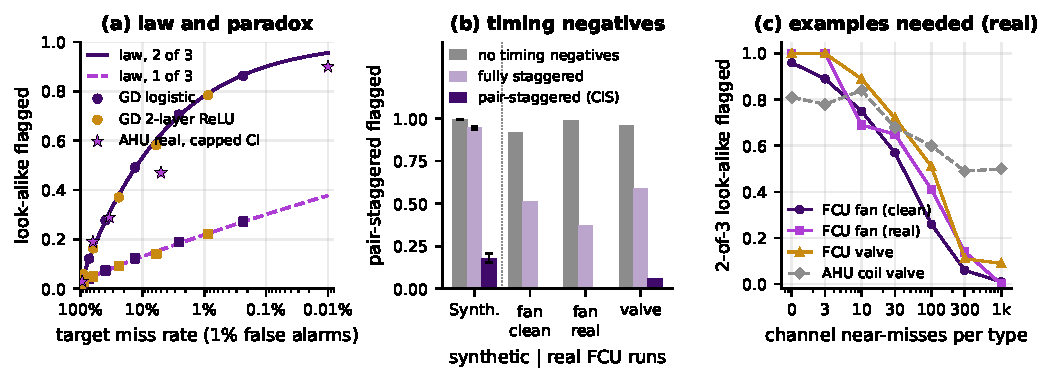
\includegraphics[width=\linewidth]{figs/fig_main.pdf}
\vspace{-14pt}
\caption{\textbf{(a)} The power--specificity curve of \cref{cor:paradox} ($k=3$, no fitted parameter) with measured 2-of-3 (circles) and 1-of-3 (squares) rates for gradient-descent logistic regression and a two-layer ReLU net over a signal sweep (5 seeds; s.d.\ smaller than markers). Stars: AHU coil-valve data, capped CI model, with the fault effect scaled by $0.05$--$1$ (one seed); miss rates below $10^{-4}$ are drawn at $10^{-4}$. \textbf{(b)} Temporal identification (\cref{thm:teach}(b,c)): flag rate on pair-staggered look-alikes after training with no timing negatives, fully staggered negatives, or pair-staggered negatives. Synthetic: raw-series two-layer net, 5 seeds (error bars: s.d.); real: LSTM on three FCU runs (one seed each). \textbf{(c)} 2-of-3 look-alike flag rate vs.\ channel near-miss examples per type (LSTM, weight decay $10^{-3}$, real data; detection stays $\ge0.99$).}
\label{fig:main}
\end{figure}

\paragraph{The law and the paradox (\cref{thm:law,cor:paradox}).} For synthetic signals, the curve evaluated at each model's \emph{own} detection rate predicts its look-alike rates. For logistic regression the largest deviation over $\delta/\sigma\in[0.5,3]$ is $0.007$ for 2-of-3 and $0.006$ for 1-of-3. The two-layer net follows the same curve with largest deviation $0.023$ (\cref{fig:main}a, \cref{tab:law}), so its learned score behaves like a sum. Detection and look-alike alarms rise together, which is the paradox. In the toy replica (\cref{tab:toyall}), the raw-series MLP, LSTM and channel-independent models lie within $0.05$ of the curve at their own detection rates ($0.94$--$0.97$). Logistic regression on window statistics lies $0.06$--$0.07$ above it and flags half of the fully staggered windows, consistent with the timing-blindness of window statistics (\cref{lem:blind}). The capped CI model and the reference rule lie below the curve on 2-of-3 ($0.42$ vs.\ $0.54$ and $0.21$ vs.\ $0.52$), as detectors that do not sum should. On real AHU data, scaling the fault effect raises the capped CI model's detection from $0.06$ to $1.00$ and its 2-of-3 alarms from $0.03$ to $0.90$ (stars). The stars follow the curve up to detection $0.66$ and fall below it at higher detection ($0.47$ vs.\ $0.63$ at detection $0.95$), consistent with capping. On the FCU, detection is already $1.00$ at a fault effect of $\times0.25$, so the paradox cannot be resolved there.

\paragraph{Composite null and capped evidence (\cref{thm:composite}).} In simulation ($k=3$), additive detectors calibrated on normal data have false-alarm rates of $0.49$--$1.00$ on near-misses. The IU detector is valid (size $0.010$), and its power $0.05/0.42/0.87/0.99$ at $\delta/\sigma=2/3/4/5$ matches $\Phi(\delta/\sigma-z_\alpha)^3$ (\cref{tab:composite}). Empirically, the capped CI model is far less sensitive to one loud sensor than the uncapped CI model (BIG1, no remedy: $0.09$ vs.\ $0.99$ in the toy). On real data, however, it did not learn the conjunction even with 1000 near-misses per type (FCU 2-of-3 rate $0.99$). Representability (\cref{thm:composite}(e)) is not learnability.

\paragraph{Separated regime (\cref{thm:sep}).} Two-layer ReLU nets trained on well-separated normal and target clusters ($k=2,\dots,8$; \cref{tab:sep}) place channel near-misses at $p=0.57$--$0.91$ of the way to the target. This is slightly above the linear limit $(k-1)/k$ and above the bound of \cref{thm:sep}(a) evaluated with the measured $R/R_{\min}\in[1.19,1.34]$. The near-misses are flagged in 98--100\% of draws. After retraining with 100 near-misses per type, path norms are $4.0$--$8.6$ times the minimum, above the requirement $k\gamma/G$ of \cref{thm:sep}(b) in every run. Even so, the fraction of near-misses still flagged grows from $0.20$ at $k=2$ to $1.00$ at $k=8$. At a fixed training budget, rejecting more near-miss types is harder, which is consistent with the growing norm cost, although this experiment does not isolate the cause.

\begin{table}[t]
\centering
\caption{Toy replica: flag rates at 1\% false alarms (mean $\pm$ s.d., 3 seeds) for each training remedy, LSTM. All remedies add the same number of label-0 windows. The fault effect moved to unrelated sensors (OFF) is flagged at $\le0.02$ under every remedy.}
\label{tab:toy}
\small
\setlength{\tabcolsep}{3pt}
\begin{tabular}{lcccccc}
\toprule
Training & Detection & 1-of-3 & 2-of-3 & BIG1 & Fully stag. & Pair-stag.\\
\midrule
Normal vs.\ target only & 0.94$\pm$0.02 & 0.13$\pm$0.00 & 0.55$\pm$0.03 & 0.65$\pm$0.08 & 0.14$\pm$0.02 & 0.27$\pm$0.02\\
+ fully staggered negatives & 0.95$\pm$0.01 & 0.06$\pm$0.01 & 0.40$\pm$0.05 & 0.08$\pm$0.04 & 0.02$\pm$0.01 & 0.12$\pm$0.05\\
+ generic negatives (OE-style) & 0.93$\pm$0.01 & 0.13$\pm$0.00 & 0.56$\pm$0.01 & 0.70$\pm$0.03 & 0.13$\pm$0.01 & 0.26$\pm$0.04\\
+ channel near-misses & 0.83$\pm$0.06 & 0.04$\pm$0.02 & 0.15$\pm$0.05 & 0.01$\pm$0.02 & 0.04$\pm$0.02 & 0.08$\pm$0.04\\
+ CIS (channel + pair-staggered) & 0.90$\pm$0.00 & 0.05$\pm$0.01 & 0.23$\pm$0.03 & 0.04$\pm$0.03 & 0.03$\pm$0.02 & 0.04$\pm$0.02\\
\midrule
Reference all-sensors rule & 0.89$\pm$0.03 & 0.05$\pm$0.01 & 0.21$\pm$0.04 & 0.05$\pm$0.02 & 0.09$\pm$0.03 & 0.33$\pm$0.06\\
\bottomrule
\end{tabular}

\end{table}

\paragraph{Which negatives teach what (\cref{thm:teach}).} In the synthetic temporal experiment (\cref{fig:main}b), fully staggered negatives remove fully staggered false alarms but leave pair-staggered look-alikes high. Pair-staggered negatives remove both, as \cref{thm:teach}(b,c) predicts. The same ordering holds on all three real FCU runs: pair-staggered look-alikes are flagged at $0.37$--$0.59$ after fully staggered negatives vs.\ $0.00$--$0.06$ after CIS, with detection at $1.00$. Fully staggered negatives do lower pair-staggered alarms partly (from $0.92$--$0.99$ on the FCU). \Cref{thm:teach}(c) does not exclude this: it says these labels do not identify simultaneity, not that a learner cannot generalize from them. In the toy replica (\cref{tab:toy}), fully staggered negatives remove fully staggered alarms ($0.14\to0.02$). Because each of their segments shifts a single sensor, they also remove most single-sensor alarms (BIG1 $0.65\to0.08$), but they leave 2-of-3 at $0.40$. Channel near-misses bring 2-of-3 to $0.15$ at a detection cost ($0.94\to0.83$). CIS reaches 2-of-3 $0.23$ and pair-staggered $0.04$ at detection $0.90$. This is close to the reference rule on 2-of-3 ($0.21$) and better on pair-staggered windows ($0.33$). Generic negatives on unrelated sensors leave every rate unchanged (2-of-3 $0.56$). They carry no information about the conjunction, unlike outlier exposure in standard OOD detection. \Cref{tab:toyremedy} shows the same ordering for all seven toy models.

\paragraph{How many examples (\cref{prop:samples}).} Near-miss sweeps on real data (\cref{fig:main}c) show that about 300 examples per type bring FCU 2-of-3 alarms from $0.96$--$1.00$ to $0.06$--$0.14$. On the AHU coil-valve target, whose third signature sensor moves only $0.37$ s.d., 1000 per type still leave $0.50$. \Cref{prop:samples} predicts this weak-sensor bottleneck: relative to a sensor moving one s.d., it implies roughly $(1/0.37)^2\approx7$ times more examples. In the synthetic sweep (\cref{tab:recipe}), stronger weight decay slows the decrease ($0.46$ vs.\ $0.34$ at 256 per type), in the direction of \cref{prop:pstar}. On real data the ordering reverses: the LSTM with weight decay $10^{-3}$ needs fewer near-misses than without (FCU fan, clean: $0.06$ vs.\ $0.44$ at 300 per type). \Cref{prop:pstar} concerns the regularized optimum of a two-layer net and does not describe this case.

\begin{table}[t]
\centering
\caption{Real faults (LBNL simulations, LSTM, one seed). \emph{2-of-3}: look-alike flag rate after normal-vs-target training (reference all-sensors rule in brackets) and after adding channel near-misses (+\,NM). \emph{Pair-stag.}: after fully staggered negatives vs.\ after CIS. \emph{Never-seen}: other fault files sharing one or two signature sensors vs.\ none. \emph{Fleet share}: fraction of false alarms caused by other faults in an 89/1/10\% normal/target/other mix.}
\label{tab:real}
\small
\setlength{\tabcolsep}{3.2pt}
\begin{tabular}{@{}lcccccc@{}}
\toprule
 & & \multicolumn{2}{c}{2-of-3 flagged} & Pair-stag.\ flagged & Never-seen faults & Fleet\\
\cmidrule(lr){3-4}\cmidrule(lr){5-5}\cmidrule(lr){6-6}
Target (signature shifts, s.d.) & Det. & plain (ref.) & + NM & stag.\,/\,CIS & partial\,/\,none & share\\
\midrule
FCU fan outlet, clean (2.6, 2.3, 1.7) & 1.00 & 0.97 (0.35) & 0.01 & 0.51 / 0.00 & 0.70 / 0.22 & 76\% \\
FCU fan outlet, real-mode & 1.00 & 1.00 (0.30) & 0.01 & 0.37 / 0.00 & 0.67 / 0.25 & 72\% \\
FCU cooling valve (9.0, 8.1, 2.3) & 1.00 & 1.00 (0.43) & 0.23 & 0.59 / 0.06 & 0.60 / 0.18 & 85\% \\
AHU coil valve (1.8, 0.8, 0.37) & 1.00 & 0.78 (0.74) & 0.30 & 0.18 / 0.15$^\dagger$ & 0.03 / 0.00 & 33\% \\
AHU damper (2.1, 0.9, 0.6) & 1.00 & 0.79 & 0.19 & -- & 0.06 / 0.01 & -- \\
\bottomrule
\end{tabular}\\[2pt]
{\footnotesize $^\dagger$Even the reference rule flags 0.90 of AHU coil PAIRSTAG windows, so the timing test is uninformative there. ``--'': not run with the new constructs.}
\end{table}

\paragraph{Real never-seen faults.} On the FCU, faults that share signature sensors are flagged far more often than faults that share none (\cref{tab:real}). Most fleet false alarms (72--85\%) then come from other faults, not from normal operation. On the AHU, other faults rarely move the sensors that the LSTM relies on, and false alarms on never-seen faults stay $\le6\%$. The law predicts exactly this: what matters is the overlap $r$ that real look-alikes have with the evidence the model sums. Adding 2-of-3 near-misses to FCU fan-outlet training also cuts flag rates on never-seen faults sharing one or two sensors, from $0.63/0.79$ to $0.11/0.22$, although none of these faults was used in training. Across $n\in\{500,2000,8000\}$ and prevalences $\{0.1,0.5,0.9\}$ the LSTM's 2-of-3 rate never fell below $0.65$ on any target, as \cref{thm:np}(ii--iii) predicts for more data and rebalancing.

\paragraph{Limitations.} The real data are simulations with less sensor noise than field data. The signature and the reference rule are estimates, and real-data runs use one seed. \Cref{thm:np,thm:law,thm:composite} assume Gaussian noise and a known onset. \Cref{thm:sep} is a bound in terms of a measured constant, not a convergence theorem for gradient descent. \Cref{thm:teach} assumes per-axis monotone learners. Where real detection saturates, the law cannot be tested quantitatively. The weight-decay prediction of \cref{prop:pstar} did not transfer to the real-data LSTM.

%=====================================================================
\section{Conclusion}
\label{sec:conclusion}
Detectors trained on normal-vs-target data learn to add up the right evidence instead of requiring all of it. For the training question this is optimal. For deployment it is wrong, and more data cannot change it. The theory gives three practical consequences. A model's look-alike false alarms can be predicted from its detection rate. Uncapped additive and channel-independent designs cannot be made safe against loud look-alikes. And the fix is small and specific: $k$ channel near-misses and $\binom k2$ pair-staggered near-misses, with the weakest sensor setting the amount. Open problems include a gradient-descent convergence theorem for non-symmetric data, the unknown-onset version of the law, and training procedures that make capped models learn the conjunction they can represent.

\bibliography{refs}
\bibliographystyle{iclr2027_conference}

\newpage
\appendix
\section{Proofs}
\label{app:proofs}
Throughout, $\Phi$ and $\varphi$ are the standard normal CDF and density, $z_\alpha=\Phi^{-1}(1-\alpha)$, and $\|\cdot\|$ is the Euclidean norm. We use two elementary facts.

\textbf{(F1)} If $x\sim\cN(\mu,\Sigma)$ and $u\in\R^d$, then $u^\top x\sim\cN(u^\top\mu,\,u^\top\Sigma u)$.

\textbf{(F2)} (Neyman--Pearson lemma, \citealp{neyman1933,lehmann2005}.) For two distributions with densities $p_0,p_1$, a test that rejects when $p_1/p_0$ exceeds a constant chosen to give size $\alpha$ is most powerful among all tests of size $\le\alpha$. Ties occur with probability $0$ when the likelihood ratio has a continuous distribution.

\subsection{Proof of \texorpdfstring{\cref{thm:np}}{Theorem 1}}
\textbf{(i)} Under \cref{ass:gauss} the densities are $p_h(x)=(2\pi)^{-d/2}|\Sigma|^{-1/2}\exp(-\frac12(x-h)^\top\Sigma^{-1}(x-h))$. Hence
\[
\log\frac{p_g(x)}{p_0(x)}=-\tfrac12(x-g)^\top\Sigma^{-1}(x-g)+\tfrac12x^\top\Sigma^{-1}x=g^\top\Sigma^{-1}x-\tfrac12g^\top\Sigma^{-1}g .
\]
By Bayes' rule the log posterior odds equal the log-likelihood ratio plus $\log\frac{\pi}{1-\pi}$, which gives $\ell_\pi$. If $\Sigma=\mathrm{blockdiag}(\Sigma_{11},\dots,\Sigma_{CC})$ over channels, then $g^\top\Sigma^{-1}x=\sum_{j}g_j^\top\Sigma_{jj}^{-1}x_j$, where $x_j,g_j\in\R^T$ are the channel-$j$ blocks. This is a sum of per-channel terms, and $g_j=0$ for $j\notin S$.

\textbf{(ii)} By (i) the likelihood ratio is a strictly increasing function of $u(x)=g^\top\Sigma^{-1}x$. By (F2), the most powerful size-$\alpha$ test rejects when $u(x)>t$, with $t$ chosen so that $P_0(u>t)=\alpha$. By (F1), under $P_0$, $u\sim\cN(0,g^\top\Sigma^{-1}\Sigma\Sigma^{-1}g)=\cN(0,D^2)$, so $t=z_\alpha D$. Neither the test nor its threshold involves $\pi$.

\textbf{(iii)} Let $P_\pi=(1-\pi)P_0+\pi P_g$ and let $\hat t_n$ be the $(1-\alpha)$-quantile of $\hat f_n$ under $P_0$. Let $t^*$ be the $(1-\alpha)$-quantile of $\ell_\pi$ under $P_0$. Since $\ell_\pi$ is an increasing affine function of $u$, $\{\ell_\pi>t^*\}=\{\phi^*=1\}$ by (ii).

\emph{Step 1 (convergence under $P_0$).} $P_0(A)\le P_\pi(A)/(1-\pi)$ for every event $A$, so $\hat f_n\to\ell_\pi$ in $P_\pi$-probability implies convergence in $P_0$-probability.

\emph{Step 2 (threshold convergence).} Let $F_n$ and $F$ be the CDFs of $\hat f_n$ and $\ell_\pi$ under $P_0$. Convergence in probability implies convergence in distribution, so $F_n(t)\to F(t)$ at every $t$, because $F$ is continuous: $\ell_\pi$ is Gaussian under $P_0$ with positive variance $D^2$. $F$ is also strictly increasing. Fix $\epsilon>0$. Then $F(t^*-\epsilon)<1-\alpha<F(t^*+\epsilon)$, and for $n$ large $F_n(t^*-\epsilon)<1-\alpha<F_n(t^*+\epsilon)$. Hence $\hat t_n\in[t^*-\epsilon,t^*+\epsilon]$, where $\hat t_n=\inf\{t:F_n(t)\ge1-\alpha\}$. So $\hat t_n\to t^*$. If $\hat t_n$ is instead the empirical quantile of $m_n\to\infty$ normal scores drawn independently of training, then conditionally on $\hat f_n$ these scores are i.i.d.\ with CDF $F_n$, and the Dvoretzky--Kiefer--Wolfowitz inequality \citep{massart1990} gives $\Pr(\sup_t|\hat F_{m_n}-F_n|>\epsilon')\le2e^{-2m_n\epsilon'^2}$ uniformly in $\hat f_n$. Taking $\epsilon'$ below the two gaps $|F_n(t^*\pm\epsilon)-(1-\alpha)|$, which stay bounded away from $0$ for large $n$, the same sandwich holds for $\hat F_{m_n}$ with probability $\to1$, so $\hat t_n\to t^*$ in probability.

\emph{Step 3 (transfer to $Q$).} $P_\pi$ has an everywhere positive density, so Lebesgue measure is absolutely continuous w.r.t.\ $P_\pi$. Hence $Q\ll P_\pi$. For finite measures this means: for every $\eta>0$ there is $\gamma>0$ with $P_\pi(A)<\gamma\Rightarrow Q(A)<\eta$. Therefore $\hat f_n\to\ell_\pi$ in $Q$-probability.

\emph{Step 4 (disagreement).} For any $\epsilon>0$, the event $\{\hat\phi_n\ne\phi^*\}$ is contained in
\[
\{|\ell_\pi-t^*|\le2\epsilon\}\ \cup\ \{|\hat f_n-\ell_\pi|>\epsilon\}\ \cup\ \{|\hat t_n-t^*|>\epsilon\}.
\]
To see this, suppose $|\ell_\pi-t^*|>2\epsilon$, $|\hat f_n-\ell_\pi|\le\epsilon$ and $|\hat t_n-t^*|\le\epsilon$. Then $\hat f_n-\hat t_n$ and $\ell_\pi-t^*$ have the same sign, so the two tests agree. The third event has probability $\to0$ (Step 2; it is eventually empty for the population quantile). The second has $Q$-probability $\to0$ (Step 3). The first has $Q$-probability $\to0$ as $\epsilon\to0$, because $\ell_\pi$ is a non-constant affine function of $x$ and so its level sets have Lebesgue measure zero, hence $Q$-measure zero. Taking $n\to\infty$ and then $\epsilon\to0$ gives $Q(\hat\phi_n\ne\phi^*)\to0$. \qed

\begin{remark}
Logistic regression on $(x,1)$ is well specified by (i), and its maximum-likelihood estimator is consistent, so it satisfies the premise of (iii). The same conclusion holds for exponential-family noise whose sufficient statistics are channel-separable: the log-likelihood ratio is then a sum of per-channel terms.
\end{remark}

\subsection{Proof of \texorpdfstring{\cref{thm:law}}{Theorem 2} and \texorpdfstring{\cref{cor:paradox}}{Corollary 3}}
Under $\cN(h,\Sigma)$, (F1) gives $u=g^\top\Sigma^{-1}x\sim\cN(g^\top\Sigma^{-1}h,\,D^2)=\cN(D^2r(h),D^2)$. Thus $\Pr_h(u>z_\alpha D)=\Pr(Z>z_\alpha-Dr(h))=\Phi(Dr(h)-z_\alpha)$ for $Z\sim\cN(0,1)$.

\emph{Special cases.} Assume independent channels with equal per-channel detectability $D_j^2=D^2/k$ for $j\in S$. For $h=g\odot\1_A$, block-diagonality gives $g^\top\Sigma^{-1}h=\sum_{j\in A}D_j^2=|A|D^2/k$, so $r=m/k$ when $|A|=m$. Shifting only channel $c$, by $c'$ times its target shift ($h=c'g_c$), gives $r=c'D_c^2/D^2=c'/k$. For $h=-g$, $r=-1$. For $h$ supported on $S^c$, $g^\top\Sigma^{-1}h=0$ because $g$ vanishes off $S$ and $\Sigma^{-1}$ is block-diagonal, so the rate is $\Phi(-z_\alpha)=\alpha$.

\emph{\Cref{cor:paradox}.} $\beta=\Phi(D-z_\alpha)$ gives $D=\Phi^{-1}(\beta)+z_\alpha$. Substituting this into the law gives the stated formula. For $r\in(0,1)$ the argument $r(\Phi^{-1}(\beta)+z_\alpha)-z_\alpha$ is strictly increasing in $\beta$ and tends to $+\infty$ as $\beta\to1$. $\Phi$ is strictly increasing. Replacing $(g,h,\Sigma)$ by $(cg,ch,\Sigma)$ with $c>1$, or by $(g,h,c\Sigma)$ with $c<1$, leaves $r(h)=g^\top\Sigma^{-1}h/g^\top\Sigma^{-1}g$ unchanged and multiplies $D$ by $c$ or $c^{-1/2}$, so $\beta$ and every look-alike rate with $r(h)\in(0,1)$ increase. \qed

\subsection{Shift statistic and proof of \texorpdfstring{\cref{thm:composite}}{Theorem 4}}
\begin{lemma}[Shift statistic]\label{lem:shift}
Let $B,I\subset[T]$ be disjoint baseline and post-onset index sets and $c=\1_I/|I|-\1_B/|B|\in\R^T$. Let $a_j=s_j\,c^\top x_j$. Under \cref{ass:gauss} with block-diagonal $\Sigma$ and a pattern $h$ whose channel-$j$ block equals $s_j\mu_j\1_I$ (and $0$ on $B$), the vector $a=(a_j)_{j\in S}$ is $\cN(\mu,\mathrm{diag}(\sigma_j^2))$ with $\sigma_j^2=c^\top\Sigma_{jj}c$.
\end{lemma}
\begin{proof}
$a_j=s_jc^\top x_j$ is linear in $x_j$, with mean $s_jc^\top(s_j\mu_j\1_I)=\mu_j$ because $c^\top\1_I=1$ and $s_j^2=1$. Its variance is $c^\top\Sigma_{jj}c$ (F1). The $a_j$ are jointly Gaussian and depend on different blocks, so block-diagonality makes them independent.
\end{proof}

\textbf{(a)} Fix $j\in S$ and let $\mu^{(j)}=\mu-\mu_je_j$, i.e.\ the near-miss without sensor $j$, with $\mu=(\delta_i)_{i\in S}$. Since $M_i\ge\delta_i$, $\cN(\mu^{(j)},\cdot)$ belongs to $\mathcal N(M)$. A deployment-valid $\phi$ is therefore in particular a level-$\alpha$ test of $\cN(\mu^{(j)},\Lambda)$ against $\cN(\mu,\Lambda)$, with $\Lambda=\mathrm{diag}(\sigma_i^2)$. These two laws differ only in the mean of coordinate $j$. By (i) of \cref{thm:np} applied to $g=\mu-\mu^{(j)}=\delta_je_j$, the log-likelihood ratio is $\delta_j(a_j-\mu^{(j)}_j)/\sigma_j^2$ plus a constant. By (F2) the most powerful level-$\alpha$ test rejects when $a_j>z_\alpha\sigma_j$, with power $\Phi(\delta_j/\sigma_j-z_\alpha)$. So no deployment-valid test exceeds this power. Minimize over $j$. \emph{Full windows:} the same argument applies to any measurable function of the whole window $x$. The target pattern $g$ and the near-miss pattern $g-g_j$ differ only in the channel-$j$ block, so with block-diagonal $\Sigma$ the likelihood ratio depends on $x_j$ only, and the most powerful test has power $\Phi(D_j-z_\alpha)$ with $D_j^2=g_j^\top\Sigma_{jj}^{-1}g_j$.

\textbf{(b)} \emph{Validity.} Let $Q\in\mathcal N(\infty)$ have support $A\subsetneq S$, and pick $j\in S\setminus A$, so $\mu_j=0$ under $Q$. Then $Q(\phi_{IU}=1)\le Q(a_j/\sigma_j>z_\alpha)=\alpha$. Under normal ($\mu=0$) the same bound holds. \emph{Power.} Under the target the $a_j$ are independent with $\Pr(a_j/\sigma_j>z_\alpha)=\Phi(D_j-z_\alpha)$, so the power is $\prod_j\Phi(D_j-z_\alpha)$. \emph{Approximation.} Write $q_j=\Phi(z_\alpha-D_j)$ for the per-coordinate miss. The IU miss is $1-\prod_j(1-q_j)\le\sum_jq_j\le k\max_jq_j$, using the union bound. By (a), every valid detector misses with probability at least $1-\min_j\Phi(D_j-z_\alpha)=\max_jq_j$.

\textbf{(c)} Let $w\ge0$, $w\ne0$, with equal $\delta,\sigma$ and $M_i=\delta$. For each $i$, the near-miss $\mu^{(i)}=\delta(\1-e_i)$ is in $\mathcal N(\delta)$, and $w^\top a\sim\cN(\delta(\|w\|_1-w_i),\sigma^2\|w\|^2)$ under it. Validity requires $\Pr(w^\top a>t)\le\alpha$, i.e.\ $t\ge\delta(\|w\|_1-w_i)+z_\alpha\sigma\|w\|$ for all $i$. The binding constraint is $i^*=\arg\min_iw_i$. The power is $\Phi\big((\delta\|w\|_1-t)/(\sigma\|w\|)\big)\le\Phi\big(\delta\min_iw_i/(\sigma\|w\|)-z_\alpha\big)$. Finally, $k\min_iw_i^2\le\|w\|^2$ gives $\min_iw_i\le\|w\|/\sqrt k$, with equality iff all $w_i$ are equal. Other members of $\mathcal N(\delta)$ have coordinatewise smaller means, hence smaller false-alarm rates (since $w\ge0$), so they do not tighten the constraint.

\textbf{(d)} Let $\psi_j$ be nondecreasing, real-valued and unbounded above. Since $k\ge2$, the vector $Ae_j$ (all sensors normal except $j$, shifted by $A>0$) has support $\{j\}\subsetneq S$, so it belongs to $\mathcal N(\infty)$ for every $A$. Fix any $t\in\R$ and $\epsilon>0$. The random variable $Y=\sum_{i\ne j}\psi_i(a_i)$ has a fixed distribution under these alternatives and is a.s.\ finite, so there is $y_\epsilon$ with $\Pr(Y<-y_\epsilon)<\epsilon$. Since $\psi_j$ is unbounded and nondecreasing, there is $u_\epsilon$ with $\psi_j(u)>t+y_\epsilon$ for all $u\ge u_\epsilon$. Under $Ae_j$, $\Pr(a_j\ge u_\epsilon)\to1$ as $A\to\infty$. Hence $\liminf_{A\to\infty}\Pr(\sum_i\psi_i(a_i)>t)\ge1-\epsilon$. So no finite threshold is valid, and the only valid choice $t=+\infty$ (never alarm) has power $0$. Linear detectors with $w_j>0$ are the case $\psi_j(u)=w_ju$. For a channel-independent model $f(X)=\sum_jf_j(X_{\cdot j})$, apply the same argument with the null member that shifts channel $j$ by $A\,s_j\1_I$. ``Unbounded along fault-direction shifts'' means $f_j(X_{\cdot j}+As_j\1_I)\to\infty$ in probability as $A\to\infty$.

\textbf{(e)} With $\psi_j=\1\{a_j>z_\alpha\sigma_j\}$ and $t=k-\frac12$, $\sum_j\psi_j>t$ iff all indicators equal $1$, i.e.\ $\phi_{IU}=1$.

\textbf{(f)} Apply \cref{thm:law} with $r=(k-1)/k$ and $D=\sqrt k\,\delta/\sigma$: $Dr=(k-1)\delta/(\sigma\sqrt k)>0$, so the rate exceeds $\Phi(-z_\alpha)=\alpha$. \qed

\subsection{Norms, Lipschitz constants, and proof of \texorpdfstring{\cref{thm:sep}}{Theorem 5}}
\begin{lemma}[Norms bound the Lipschitz constant]\label{lem:lip}
For $f(x)=\sum_iv_i\sigma(w_i^\top x+b_i)+c$ with $\sigma$ 1-Lipschitz, $|f(x)-f(y)|\le R\|x-y\|$ with $R=\sum_i|v_i|\|w_i\|$. Moreover, $\min$ over the per-unit rescalings $(v_i,w_i,b_i)\mapsto(v_i/s,sw_i,sb_i)$, $s>0$, of $\frac12\sum_i(v_i^2+\|w_i\|^2+b_i^2)$ is at least $R$. For ReLU these rescalings leave $f$ unchanged, so $\ell_2$ weight decay upper-bounds $\lambda R$ at any minimizer. For depth-$L$ networks, $\Lip(f)\le\prod_l\|W_l\|_{\mathrm{op}}\le(\|\theta\|^2/L)^{L/2}$.
\end{lemma}
\begin{proof}
$|f(x)-f(y)|\le\sum_i|v_i||\sigma(w_i^\top x+b_i)-\sigma(w_i^\top y+b_i)|\le\sum_i|v_i||w_i^\top(x-y)|\le R\|x-y\|$ by Cauchy--Schwarz. For one unit, $\min_{s>0}\frac12(v^2/s^2+s^2(\|w\|^2+b^2))=|v|\sqrt{\|w\|^2+b^2}\ge|v|\|w\|$, by AM--GM with equality at $s^2=|v|/\sqrt{\|w\|^2+b^2}$. ReLU is positively homogeneous, so the rescaling preserves $f$. For depth $L$, the Lipschitz constant of a composition is at most the product of the factors' constants. Then $\|W_l\|_{\mathrm{op}}\le\|W_l\|_F$, and AM--GM gives $\prod_l\|W_l\|_F\le(\sum_l\|W_l\|_F^2/L)^{L/2}$.
\end{proof}

\textbf{\Cref{thm:sep}(a).} By definition of the Lipschitz constant, $f(x)\ge f(x_+)-\Lip(f)\|x-x_+\|=f(x_+)-\kappa\frac{G}{\Delta}\rho\Delta=f(x_+)-\kappa\rho G$. Subtracting $f(x_0)$ and dividing by $G$ gives $p(x)\ge1-\kappa\rho$. \emph{Distances.} Take $x_0=0$ (baseline-corrected normal) and $x_+=g$, with every signature channel shifted by $\delta$ on a block $\mathcal B$ of $L$ steps. Then $\Delta=\delta\sqrt{kL}$. The channel-$j$ near-miss $x^{(j)}=g-g_j$ satisfies $\|x^{(j)}-x_+\|=\|g_j\|=\delta\sqrt L$, so $\rho=1/\sqrt k$. Displacing channel $j$'s block by $\Delta t\le L$ steps changes $\Delta t$ entries from $\delta$ to $0$ and $\Delta t$ entries from $0$ to $\delta$, so the distance is $\delta\sqrt{2\Delta t}$ and $\rho=\sqrt{2\Delta t/(kL)}$. \emph{Interpretation of $\kappa$.} Every $f$ with $f(x_+)-f(x_0)=G$ has $\Lip(f)\ge G/\Delta$, and the linear score $f(x)=\frac{G}{\Delta^2}(x_+-x_0)^\top(x-x_0)$ attains it. So $\kappa\ge1$ measures excess slope. In experiments we upper-bound $\kappa$ by $R/R_{\min}$ using \cref{lem:lip}.

\textbf{\Cref{thm:sep}(b).} For each unit and each $j$,
$|\relu(w_i^\top x_++b_i)-\relu(w_i^\top x^{(j)}+b_i)|\le|w_i^\top(x_+-x^{(j)})|=\delta|\sum_{t\in\mathcal B}w_{i,tj}|\le\delta\sum_{t\in\mathcal B}|w_{i,tj}|$, where $w_{i,tj}$ is the weight of unit $i$ on input $(t,j)$. Summing over units with weights $|v_i|$ gives $\gamma\le f(x_+)-f(x^{(j)})\le\delta\sum_i|v_i|\sum_{t\in\mathcal B}|w_{i,tj}|$. Summing over $j\in S$,
\[
k\gamma\le\delta\sum_i|v_i|\,\|w_{i,\mathcal B\times S}\|_1\le\delta\sqrt{kL}\sum_i|v_i|\,\|w_{i,\mathcal B\times S}\|_2\le\delta\sqrt{kL}\,R ,
\]
using Cauchy--Schwarz on the $kL$ coordinates of $\mathcal B\times S$. Hence $R\ge\sqrt k\gamma/(\delta\sqrt L)$. With $R_{\min}=G/\Delta=G/(\delta\sqrt{kL})$ this is $R\ge k\frac{\gamma}{G}R_{\min}$. For unequal shifts the same steps give $R\ge\gamma\sum_{j\in S}\delta_j^{-1}/\sqrt{kL}$. \qed

\begin{remark}[Exact linear limit]\label{rem:lyu}
\citet{lyu2021} show that, for linearly separable data that is symmetric (closed under $(x,y)\mapsto(-x,-y)$), gradient flow from small initialization on two-layer leaky-ReLU networks converges in direction to the linear max-margin classifier. Symmetry holds exactly after centring at the midpoint of the prototypes and symmetrizing the sample. For two prototypes $\pm(x_+-x_0)/2$ that classifier is proportional to $x_+-x_0\propto\1_S$ (in shift-statistic space), so channel near-misses sit at $p=(k-1)/k$. The midpoint threshold is $p=\frac12$, which they exceed for every $k\ge3$. We do not rely on this result for non-symmetric data. \Cref{thm:sep} holds for any network, in terms of its measured $\kappa$.
\end{remark}

\begin{proposition}[Necessary near-miss fraction under weight decay]\label{prop:pstar}
In shift-statistic space, take noise-free prototypes with mass $q$ at $x_0=0$ (label $-1$), $q$ at $x_+=\delta\1_S$ (label $+1$), and $p/k$ at each channel near-miss (label $-1$), with $2q+p=1$. Let $\ell(z)=\log(1+e^{-z})$ and consider two-layer ReLU networks with objective $J(\theta)=\sum\mathrm{mass}\cdot\ell(yf_\theta(x))+\lambda R(\theta)$. Define
\begin{align*}
J_{\mathrm{cheap}}(p)&=\min_{m_0,m_1\ge0}\ q\ell(m_0)+q\ell(m_1)+p\,\ell\big(-m_1+\tfrac{m_0+m_1}{k}\big)+\lambda\tfrac{m_0+m_1}{\delta\sqrt k},\\
B(p)&=\inf_{m,m_0\in\R}\ q\ell(m)+q\ell(m_0)+\lambda\max\Big(\tfrac{\sqrt k\,m_+}{\delta},\tfrac{|m+m_0|}{\delta\sqrt k}\Big).
\end{align*}
If $J_{\mathrm{cheap}}(p)<B(p)$, every minimizer of $J$ flags at least one near-miss ($f(x^{(j)})>0$). The same holds with $\lambda R$ replaced by $\ell_2$ weight decay $\frac{\lambda}{2}\sum_i(v_i^2+\|w_i\|^2+b_i^2)$ with an unpenalized output bias: by \cref{lem:lip} the weight decay of every $\theta$ is at least $\lambda R(\theta)$, and for the one-unit network of the upper bound, which has hidden bias $0$, the best rescaling makes it equal to $\lambda R$.
\end{proposition}
\begin{proof}
\emph{Upper bound.} The one-unit network $f(x)=v\,\relu(\1_S^\top x/\sqrt k)-m_0$ with $v=(m_0+m_1)/(\delta\sqrt k)$ has $f(x_0)=-m_0$, $f(x_+)=m_1$ and $f(x^{(j)})=v\delta(k-1)/\sqrt k-m_0=m_1-(m_0+m_1)/k$. Its path norm is $v$, since $\|\1_S/\sqrt k\|=1$. So $\min J\le J_{\mathrm{cheap}}(p)$. \emph{Lower bound.} Let $f$ reject every near-miss, $f(x^{(j)})\le0$, and write $m=f(x_+)$, $m_0=-f(x_0)$. The near-miss losses are nonnegative, so they can be dropped. \Cref{thm:sep}(b) with $\gamma=m_+$ ($L=1$) gives $R\ge\sqrt k\,m_+/\delta$. \Cref{lem:lip} with $\|x_+-x_0\|=\delta\sqrt k$ gives $R\ge|m+m_0|/(\delta\sqrt k)$. Hence $J(\theta)\ge B(p)$, and when $J_{\mathrm{cheap}}(p)<B(p)$ no near-miss-rejecting network attains $\min J$.
\end{proof}
Numerically ($\delta=1$), the largest $p$ with $J_{\mathrm{cheap}}<B$ is $p^*=2\times10^{-4},1.3\times10^{-3},8.8\times10^{-3},1.7\times10^{-2}$ for $\lambda=10^{-4},10^{-3},10^{-2},3\times10^{-2}$ at $k=3$, and $p^*$ grows with $k$ (to $6.1\times10^{-2}$ at $k=8$, $\lambda=3\times10^{-2}$). This is a \emph{necessary} condition only. With noisy data, gradient-trained networks needed far more near-misses (\cref{tab:recipe}).

\subsection{Proof of \texorpdfstring{\cref{thm:teach}}{Theorem 6}}
\textbf{Setting.} The labelled examples are configurations labelled by the target rule $h^*$. A labelled set $\mathcal L$ identifies $h^*$ within $\mathcal H$ if $h^*$ is the only $h\in\mathcal H$ with $h(c)=h^*(c)$ for all $c\in\mathcal L$. \emph{Channel axis.} Configurations are $A\subseteq S$ (sensors shifted, simultaneously). $\mathcal H_{\mathrm{ch}}$ is the set of $h:2^S\to\{0,1\}$ that are monotone ($A\subseteq A'\Rightarrow h(A)\le h(A')$) with $h(S)=1$. The target is $h^*_{\mathrm{ch}}(A)=\1\{A=S\}$, and training data label $A=\emptyset$ (normal) as $0$. \emph{Time axis.} All of $S$ is shifted on nonempty half-open intervals $I_j=[l_j,u_j)$. Configurations are the realizable overlap graphs $\mathcal G$ on vertex set $S$. $\mathcal H_{\mathrm t}$ is the set of $h$ monotone in the edge set with $h(K_k)=1$. The target ``some moment at which all $k$ are shifted'' is $h^*_{\mathrm t}$.

\textbf{(a)} \emph{Sufficiency.} Let $\mathcal L\ni\emptyset$ contain every $S\setminus\{j\}$. Any $A\ne S$ omits some $j$, so $A\subseteq S\setminus\{j\}$, and monotonicity gives $h(A)\le h(S\setminus\{j\})=0$ for every consistent $h$. Together with $h(S)=1$ this forces $h=h^*_{\mathrm{ch}}$. \emph{Necessity.} If $S\setminus\{i\}\notin\mathcal L$, let $h_i(A)=\1\{A\supseteq S\setminus\{i\}\}$. It is monotone, $h_i(S)=1$, and $h_i(\emptyset)=0$ since $k\ge2$. It differs from $h^*_{\mathrm{ch}}$ exactly at $A=S\setminus\{i\}$, so it agrees with $h^*_{\mathrm{ch}}$ on $\mathcal L$ and $\mathcal L$ does not identify. (This characterization of teaching sets for monotone rules is classical, cf.\ \citealp{goldman1995}.)

\textbf{(b)} \emph{Helly on the line.} If $I_i\cap I_j\ne\emptyset$ for all $i,j$, then $l_i<u_j$ for all $i,j$, so $\max_il_i<\min_ju_j$, and every point of $[\max_il_i,\min_ju_j)$ lies in all intervals. Conversely a common point lies in every pairwise intersection. Hence $h^*_{\mathrm t}(\mathcal G)=\1\{\mathcal G=K_k\}$, the conjunction of the $\binom k2$ edge indicators. \emph{Sufficiency.} If $\mathcal L$ contains $K_k-e$ for every edge $e$, any realizable $\mathcal G\ne K_k$ misses some edge $e$, so $\mathcal G\subseteq K_k-e$ and $h(\mathcal G)\le h(K_k-e)=0$. \emph{Necessity.} If $K_k-e\notin\mathcal L$, let $h_e(\mathcal G)=\1\{\mathcal G\supseteq K_k-e\}$. It is monotone with $h_e(K_k)=1$ and differs from $h^*_{\mathrm t}$ only at $K_k-e$, so it is consistent with $\mathcal L$. \emph{Realizability with equal durations.} For $e=\{a,b\}$ take $I_a=[0,1)$, $I_b=[1,2)$ and $I_j=[\frac12,\frac32)$ otherwise. Then $I_a\cap I_j=[\frac12,1)$, $I_b\cap I_j=[1,\frac32)$, $I_j\cap I_{j'}=I_j$ and $I_a\cap I_b=\emptyset$, so $\mathcal G=K_k-e$. (\Cref{alg:cis} uses exactly this construction scaled to the post-onset window.)

\textbf{(c)} The fully staggered configuration has $\mathcal G=\emptyset$, the minimum of the edge order. Labelling it $0$ excludes exactly the rules with $h(\emptyset)=1$. By monotonicity that is only the constant rule $h\equiv1$. For $k\ge3$, $K_k-e\ne\emptyset$, so every witness $h_e$ in the necessity proof of (b) satisfies $h_e(\emptyset)=0$ and survives. Fully staggered negatives therefore neither identify the rule nor replace any pair-staggered pattern. (For $k=2$, $K_2-e=\emptyset$ and the two notions coincide.)

\textbf{(d)} Let $\mathcal C_{\mathrm{ch}}$ and $\mathcal C_{\mathrm t}$ be the two configuration sets, sharing only the target (all $k$ sensors shifted and overlapping). Let $\mathcal H$ contain the rules on $\mathcal C_{\mathrm{ch}}\cup\mathcal C_{\mathrm t}$ whose restrictions lie in $\mathcal H_{\mathrm{ch}}$ and $\mathcal H_{\mathrm t}$. The constraints decouple, since every member equals $1$ at the shared target. So $\mathcal L$ identifies $h^*$ in $\mathcal H$ iff $\mathcal L\cap\mathcal C_{\mathrm{ch}}$ and $\mathcal L\cap\mathcal C_{\mathrm t}$ identify on their axes. By (a) and (b) this needs and is achieved by the $k$ channel and the $\binom k2$ pair-staggered near-misses. \qed

\begin{remark}[Joint monotonicity]\label{rem:joint}
Suppose instead that rules are monotone in the joint order $(A,\mathcal G)\preceq(A',\mathcal G')$ iff $A\subseteq A'$ and $\mathcal G\subseteq\mathcal G'$, over all configurations. Then the channel near-miss $(S\setminus\{j\},K_{S\setminus\{j\}})$ lies below $(S,K_k-\{i,j\})$ for any $i\ne j$. So the $\binom k2$ pair-staggered negatives would already force every channel near-miss to $0$. We do not assume joint monotonicity for learned networks, and we did not test pair-staggered negatives alone. Our real-data remedy (CIS) supplies both types.
\end{remark}

\subsection{Proof of \texorpdfstring{\cref{prop:samples}}{Proposition 7}}
Let $\bar x_j$ and $\bar y_j$ be the sample means of sensor $j$ over $n$ i.i.d.\ near-misses of type $j$ and $n$ targets, with true means $\nu_j$ and $\nu_j+\Delta_j$ and noise $\cN(0,\sigma_j^2)$. The threshold is $\hat c_j=(\bar x_j+\bar y_j)/2$, and the midpoint is $c_j=\nu_j+\Delta_j/2$. Then $|\hat c_j-c_j|\le\frac12(|\bar x_j-\nu_j|+|\bar y_j-\nu_j-\Delta_j|)\le\max(|\bar x_j-\nu_j|,|\bar y_j-\nu_j-\Delta_j|)$. The Gaussian tail bound gives $\Pr(|\bar x_j-\nu_j|>t)\le2e^{-nt^2/(2\sigma_j^2)}$, and similarly for $\bar y_j$. With $t=\Delta_j/4$, $\Pr(|\hat c_j-c_j|>\Delta_j/4)\le4e^{-n\Delta_j^2/(32\sigma_j^2)}$. A union bound over $j\in S$ shows that all thresholds are within $\Delta_j/4$ of their midpoints with probability $\ge1-4k\,e^{-n\min_j\Delta_j^2/(32\max_j\sigma_j^2)}\ge1-\eta$ under the stated condition on $n$. On this event $\hat c_j\ge\nu_j+\Delta_j/4$. A new near-miss of type $j$ is flagged only if its sensor-$j$ value exceeds $\hat c_j$, which has probability $\le\Phi(-\Delta_j/(4\sigma_j))$. Symmetrically $\hat c_j\le\nu_j+\frac34\Delta_j$, so the target fails sensor $j$ with probability $\le\Phi(-\Delta_j/(4\sigma_j))$. A union bound over $j$ bounds the miss probability. If the $n$ values are consecutive draws of a stationary AR(1) sequence with $\phi\in[0,1)$, the variance of their mean is $\frac{\sigma_j^2}{n}\big(1+2\sum_{h=1}^{n-1}(1-\frac hn)\phi^h\big)\le\frac{\sigma_j^2}{n}\frac{1+\phi}{1-\phi}$ for every $n$ (\cref{lem:ar}). The mean is still Gaussian, since it is a linear functional, so the tail bound holds with $n$ replaced by $n(1-\phi)/(1+\phi)$. \qed

\subsection{Window statistics and temporal dependence}
\begin{lemma}[Window statistics are timing- and sign-blind]\label{lem:blind}
Let $\psi:\R^T\to\R^q$ be invariant to permutations of the time index (e.g.\ mean, standard deviation, minimum, maximum, quantiles), and $\Psi(X)=(\psi(X_{\cdot1}),\dots,\psi(X_{\cdot C}))$. Suppose the noise has exchangeable time entries within each channel and independent channels. (i) If two patterns $G,G'$ have, channel by channel, the same multiset of entries, then $\Psi(W+G)\overset{d}{=}\Psi(W+G')$. In particular, simultaneous, fully staggered and pair-staggered patterns with equal per-channel durations are indistinguishable by any detector built on $\Psi$. (ii) If $W\overset d=-W$ and $\psi(-x)=\psi(x)$ (dispersion statistics), then $\psi(W+G)\overset d=\psi(W-G)$.
\end{lemma}
\begin{proof}
(i) For each $j$ choose a permutation $\pi_j$ with $G'_{\cdot j}=G_{\pi_j(\cdot),j}$. Exchangeability gives $W_{\cdot j}\overset d=W_{\pi_j(\cdot),j}$, and independence across channels makes this joint over $j$. Hence $(W+G')_{\cdot j}\overset d=(W+G)_{\pi_j(\cdot),j}$ jointly, and $\psi$ is permutation-invariant. (ii) $\psi(W+G)=\psi(-W-G)\overset d=\psi(W-G)$.
\end{proof}
With AR noise, or with order-dependent statistics such as a slope or a last-$m$ mean, (i) holds only approximately. Consistent with this, the window-statistics models flag consecutive-segment staggered faults at $0.57$--$1.00$ on the real targets of \cref{tab:realall}.

\begin{lemma}[Temporal dependence enters through the effective noise]\label{lem:ar}
For stationary noise with autocovariance $\gamma(\cdot)$, the shift statistic of \cref{lem:shift} has $\sigma_j^2=c^\top\Gamma c$ with $\Gamma_{st}=\gamma(s-t)$. For AR(1) noise with coefficient $\phi\in(-1,1)$ and marginal variance $\sigma_x^2$, the variance of an $L$-step mean is $\sigma_x^2L^{-2}\sum_{s,t}\phi^{|s-t|}$, and $L$ times this tends to $\sigma_x^2(1+\phi)/(1-\phi)$ as $L\to\infty$. All results above hold with these effective variances. For a post-onset mean against a known baseline ($c=\1_I/|I|$) and $\phi\in[0,1)$, a larger $\phi$ raises $\sigma_j^2$ and lowers $D$, which moves a detector \emph{along} the curve of \cref{cor:paradox}: detection and look-alike alarms both fall. This is not monotone for every statistic. Correlated noise partly cancels in the baseline-corrected difference, and for a unit step on the last 28 of $T=48$ steps (unit marginal variance) the full-window $D^2$ falls from $28$ at $\phi=0$ to $6.7$ at $\phi=0.9$ and rises to $50$ at $\phi=0.99$.
\end{lemma}
\begin{proof}
$a_j$ is a linear functional of $x_j$ (F1). For AR(1), $\gamma(h)=\sigma_x^2\phi^{|h|}$. Then $L\cdot L^{-2}\sum_{s,t=1}^L\phi^{|s-t|}=1+2\sum_{h=1}^{L-1}(1-h/L)\phi^h\to1+2\phi/(1-\phi)=(1+\phi)/(1-\phi)$ by dominated convergence. For $\phi\ge0$ every term is nonnegative and at most $\phi^h$, which gives the bound used in \cref{prop:samples}, and each term is nondecreasing in $\phi$, which gives the monotonicity claim.
\end{proof}

%=====================================================================
\section{Experimental details}
\label{app:exp}
\paragraph{Synthetic experiments} (code: \texttt{paper\_synth.py}, \texttt{theory\_checks.py}). All thresholds are the $0.99$ quantile of the score on $20{,}000$ fresh normal samples, and rates are estimated on $4{,}000$--$20{,}000$ fresh samples per construct. \emph{Law/paradox (S1):} $d=20$, $k=3$, $\sigma=1$, $\delta/\sigma\in\{0.5,\dots,3\}$, $2{,}000+2{,}000$ training samples. Learners: full-batch gradient-descent logistic regression ($2{,}000$ steps, step size $0.5$), and a two-layer ReLU net (64 units, initialization scale $10^{-2}$, Adam, $1{,}500$ steps, learning rate $10^{-2}$). 5 seeds. \emph{Composite (C3):} shift statistics with $k=3$, $\sigma=1$, $4\times10^5$ draws per construct; ``unbounded'' look-alikes use shifts of $50\delta$. \emph{Separated regime (S2):} $d=10$, $\sigma=0.15$, $\delta=1$, $500+500$ samples, two-layer ReLU (64 units, initialization $10^{-3}$, Adam, $3{,}000$ steps, $10^{-2}$), with 100 near-misses per type in the ``with near-misses'' runs. 3 seeds. \emph{Temporal (S3):} raw windows $T=60$, $C=6$, $k=3$, $\sigma=0.5$, $\delta=1$, shift duration $L\sim\mathcal U\{12,\dots,18\}$, random onset; $1{,}500+1{,}500$ samples plus $600$ timing negatives; two-layer ReLU on the flattened window (64 units, Adam, $1{,}200$ steps, $3\times10^{-3}$, weight decay $10^{-4}$). 5 seeds. \emph{Recipe (S4):} $d=10$, $k=3$, $\sigma=0.3$, $1{,}000+1{,}000$ samples plus $c\in\{0,4,16,64,256\}$ near-misses per type, weight decay $\in\{0,10^{-3}\}$. 3 seeds.

\paragraph{Toy replica} (\texttt{run\_toy.py}). 20 channels, 48 steps, AR(1) with $\phi=0.7$ and unit variance, a shared slow load factor ($\phi=0.97$, weight $0.6$) on channels 0--5. The target lowers channels 0, 1, 2 by $2.5$ from a random onset in $[10,25]$. The per-window baseline (mean of the first 8 steps) is subtracted. 4,000 training windows (50/50), 2,000 normal validation windows for calibration, 2,000 test windows per construct. 3 seeds (data and initialization).

\paragraph{Real data} (\texttt{real\_data.py}, \texttt{run\_real.py}). LBNL fan-coil and single-duct AHU simulations \citep{granderson2023}, each a set of one-year runs: one fault-free run and one run per fault and severity, with identical weather and schedule. Preprocessing: resampling to 15 minutes. We drop setpoint channels, channels constant in the fault-free run, and channels that shift in the same direction in $\ge80\%$ of fault families (a fault-free/faulty configuration mismatch in the AHU benchmark). Each channel is standardized by its fault-free statistics. \emph{Signature}: the $k=3$ channels with the largest mean standardized shift while the fault is visibly present, skipping near-duplicates ($|\rho|>0.98$; disabled for the AHU coil valve, where valve position and command diverge by design). A window qualifies as a training positive only if every signature channel moves by $\ge0.5$ s.d.\ ($0.3$ for the AHU coil valve) in its fault direction after onset. Windows are 48 steps (12 h), with onset uniform in $[10,25]$ and the first-8-step baseline subtracted. Train, validation and test splits use alternating 7-day blocks. Training uses 4,000 windows (50/50), with half of the normal windows time-matched to positives with the fault removed. Testing uses 1,000 windows per construct and up to 300 windows per other fault file. \emph{Clean mode} applies the fault effect only to signature channels. \emph{Real mode} keeps every channel's real deviation.

\paragraph{Models.} Window statistics: mean, min, max, s.d., slope and last-8 mean per channel. Logistic regression ($C=1$, standardized), random forest (200 trees, min leaf 2), gradient boosting (scikit-learn defaults), MLP on every 4th step (hidden $128,64$, Adam, early stopping). LSTM: 32 hidden units, BPTT, Adam ($3\times10^{-3}$), batch 64, gradient clipping 5, up to 30 epochs, early stopping on 15\% validation loss with patience 6. Channel-independent model: shared per-channel encoder $z_c=\relu(x_cW_1+b_1)$ (32 units) with a linear head $\sum_cA_c^\top z_c$. Capped CI: $\beta\sum_c\tanh(A_c^\top z_c+d_c)$, with the same encoder and a learnable $\beta$ initialized at 3. All neural models are implemented in NumPy and pass finite-difference gradient checks. \emph{Reference rule}: each signature channel minus a ridge prediction from the non-signature channels (fit on normal windows), scaled by its residual s.d., and $\max_\tau\min_{j\in S}$ of the 8-step window means after step 8. Calibrated like the models.

\paragraph{Remedies.} Each fix adds $n_{\mathrm{train}}/2=2{,}000$ label-0 windows: channel near-misses (all-but-one, cycling over the left-out channel); fully staggered (half ``consecutive segments'', half ``separate short dips''); CIS (half channel near-misses, half pair-staggered, cycling over pairs); generic negatives (the fault's effect moved onto $k$ unrelated channels). The recipe sweep adds $c\in\{0,3,10,30,100,300,1000\}$ near-misses per type to an otherwise identical training set. The signal sweep multiplies $D$ by a factor in both training and test.

\paragraph{Compute.} All experiments run on a 2-core CPU. The synthetic suite takes about 30 minutes, one toy seed about 10 minutes, and one real-data target 10--60 minutes.

%=====================================================================
\section{Additional results}
\label{app:more}
\begin{table}[h]\centering\small
\caption{Synthetic law check (S1; mean$\pm$s.d., 5 seeds). \emph{Law}: \cref{cor:paradox} evaluated at the model's own measured detection rate (no fitting).}\label{tab:law}
\setlength{\tabcolsep}{3pt}\begin{tabular}{llccccc}\toprule
Model & $\delta/\sigma$ & Detection & 2-of-3 & law & 1-of-3 & law\\\midrule
GD logistic & 0.5 & 0.070$\pm$0.005 & 0.040$\pm$0.003 & 0.039 & 0.021$\pm$0.002 & 0.021\\
 & 1.0 & 0.274$\pm$0.012 & 0.122$\pm$0.007 & 0.120 & 0.041$\pm$0.003 & 0.040\\
 & 1.5 & 0.606$\pm$0.015 & 0.278$\pm$0.012 & 0.276 & 0.074$\pm$0.004 & 0.072\\
 & 2.0 & 0.869$\pm$0.011 & 0.491$\pm$0.017 & 0.489 & 0.123$\pm$0.007 & 0.120\\
 & 2.5 & 0.974$\pm$0.002 & 0.706$\pm$0.013 & 0.699 & 0.190$\pm$0.009 & 0.184\\
 & 3.0 & 0.998$\pm$0.000 & 0.863$\pm$0.006 & 0.867 & 0.273$\pm$0.010 & 0.272\\
GD 2-layer ReLU & 0.5 & 0.026$\pm$0.004 & 0.019$\pm$0.002 & 0.019 & 0.014$\pm$0.001 & 0.014\\
 & 1.0 & 0.113$\pm$0.007 & 0.059$\pm$0.005 & 0.057 & 0.027$\pm$0.002 & 0.025\\
 & 1.5 & 0.379$\pm$0.026 & 0.164$\pm$0.009 & 0.163 & 0.050$\pm$0.002 & 0.049\\
 & 2.0 & 0.760$\pm$0.012 & 0.370$\pm$0.009 & 0.381 & 0.093$\pm$0.004 & 0.094\\
 & 2.5 & 0.941$\pm$0.004 & 0.582$\pm$0.022 & 0.605 & 0.141$\pm$0.009 & 0.151\\
 & 3.0 & 0.991$\pm$0.003 & 0.785$\pm$0.015 & 0.793 & 0.222$\pm$0.009 & 0.226\\
\bottomrule\end{tabular}\end{table}

\begin{table}[h]\centering\small
\caption{Composite null (C3, $k=3$, $4\times10^5$ draws). \emph{Size}: worst false-alarm rate over look-alikes, with shifts bounded by $\delta$ or unbounded ($50\delta$). Additive detectors are calibrated either on normal data or for the bounded null (\cref{thm:composite}(c)).}\label{tab:composite}
\setlength{\tabcolsep}{3pt}\begin{tabular}{ccccccccc}\toprule
 & \multicolumn{3}{c}{Additive, normal-calibrated} & \multicolumn{2}{c}{Additive, bounded-null} & \multicolumn{2}{c}{Intersection-union} & Bound\\
$\delta/\sigma$ & size ($\le\delta$) & size ($\infty$) & power & size ($\infty$) & power & size ($\infty$) & power (pred.) & (a)\\\midrule
2 & 0.493 & 1.000 & 0.872 & 1.000 & 0.121 & 0.010 & 0.051 (0.052) & 0.372\\
3 & 0.872 & 1.000 & 0.998 & 1.000 & 0.276 & 0.010 & 0.423 (0.421) & 0.750\\
4 & 0.989 & 1.000 & 1.000 & 1.000 & 0.493 & 0.010 & 0.866 (0.865) & 0.953\\
5 & 1.000 & 1.000 & 1.000 & 1.000 & 0.712 & 0.010 & 0.989 (0.989) & 0.996\\
\bottomrule\end{tabular}\end{table}

\begin{table}[h]\centering\small
\caption{Separated regime (S2; mean$\pm$s.d., 3 seeds). Left block: normal-vs-target training. \emph{Position}: $p(x^{(j)})$ of channel near-misses at the prototypes. \emph{Bound}: $1-(R/R_{\min})/\sqrt k$, a valid lower bound on the position because $\kappa\le R/R_{\min}$ (\cref{lem:lip}). \emph{Flagged}: near-miss flag rate at 1\% false alarms. Right block: retrained with 100 near-misses per type. \emph{Norm ratio}: $R/G$ after over $R/G$ before. \cref{thm:sep}(b) requires $R/R_{\min}\ge k\gamma/G$ with $\gamma$ the smallest target-minus-near-miss score gap; it held in every run. Detection after retraining is 1.000 throughout.}\label{tab:sep}
\setlength{\tabcolsep}{3pt}\begin{tabular}{cccccc|cccc}\toprule
$k$ & linear $\frac{k-1}{k}$ & position & bound & $R/R_{\min}$ & flagged & norm ratio & $R/R_{\min}$ & $k\gamma/G$ & flagged\\\midrule
2 & 0.500 & 0.565$\pm$0.049 & 0.049 & 1.34 & 0.980 & 3.00$\pm$0.34 & 4.03 & 1.89 & 0.203\\
3 & 0.667 & 0.727$\pm$0.009 & 0.267 & 1.27 & 1.000 & 3.82$\pm$0.53 & 4.85 & 2.24 & 0.600\\
4 & 0.750 & 0.808$\pm$0.023 & 0.404 & 1.19 & 1.000 & 5.96$\pm$0.84 & 7.11 & 2.77 & 0.797\\
6 & 0.833 & 0.886$\pm$0.010 & 0.505 & 1.21 & 1.000 & 7.05$\pm$1.14 & 8.56 & 3.53 & 0.978\\
8 & 0.875 & 0.911$\pm$0.004 & 0.574 & 1.20 & 1.000 & 5.81$\pm$0.78 & 7.00 & 1.25 & 1.000\\
\bottomrule\end{tabular}\end{table}

\begin{table}[h]\centering\small
\caption{Recipe curves: 2-of-3 look-alike flag rate vs.\ channel near-misses per type. Top: synthetic two-layer ReLU (S4; mean$\pm$s.d., 3 seeds). Bottom: real data, LSTM, one seed (detection $\ge0.99$ throughout).}\label{tab:recipe}
\setlength{\tabcolsep}{3pt}\begin{tabular}{lccccccc}\toprule
Synthetic, per type & 0 & 4 & 16 & 64 & 256 & & \\\midrule
weight decay 0 & 0.87$\pm$0.03 & 0.53$\pm$0.03 & 0.48$\pm$0.17 & 0.44$\pm$0.08 & 0.34$\pm$0.03 & & \\
weight decay 0.001 & 0.93$\pm$0.00 & 0.90$\pm$0.01 & 0.77$\pm$0.05 & 0.60$\pm$0.05 & 0.46$\pm$0.03 & & \\
\midrule Real, per type & 0 & 3 & 10 & 30 & 100 & 300 & 1000\\\midrule
FCU fan (clean), wd $10^{-3}$ & 0.96 & 0.89 & 0.75 & 0.57 & 0.26 & 0.06 & 0.01\\
FCU fan (clean), wd 0 & 0.95 & 0.92 & 0.82 & 0.62 & 0.54 & 0.44 & 0.08\\
FCU fan (real), wd $10^{-3}$ & 1.00 & 1.00 & 0.69 & 0.65 & 0.41 & 0.14 & 0.00\\
FCU fan (real), wd 0 & 0.99 & 1.00 & 0.78 & 0.74 & 0.55 & 0.32 & 0.12\\
FCU valve, wd $10^{-3}$ & 1.00 & 1.00 & 0.89 & 0.72 & 0.51 & 0.11 & 0.09\\
FCU valve, wd 0 & 1.00 & 1.00 & 1.00 & 0.86 & 0.81 & 0.64 & 0.06\\
AHU coil valve, wd $10^{-3}$ & 0.81 & 0.78 & 0.84 & 0.68 & 0.60 & 0.49 & 0.50\\
AHU coil valve, wd 0 & 0.74 & 0.79 & 0.83 & 0.67 & 0.53 & 0.54 & 0.47\\
\bottomrule\end{tabular}\end{table}

\begin{table}[h]\centering\small
\caption{Toy replica, all models, normal-vs-target training (mean$\pm$s.d., 3 seeds). Columns \emph{law} give \cref{cor:paradox} at each model's mean detection rate with equal shares ($r=m/k$).}\label{tab:toyall}
\setlength{\tabcolsep}{2.5pt}\resizebox{\linewidth}{!}{\begin{tabular}{lcccccccccc}\toprule
Model & Detection & 1-of-3 & law & 2-of-3 & law & BIG1 & Fully st. & Pair-st. & UP & OFF\\\midrule
LogReg (stats) & 0.98$\pm$0.00 & 0.26$\pm$0.04 & 0.19 & 0.79$\pm$0.02 & 0.73 & 1.00$\pm$0.00 & 0.51$\pm$0.07 & 0.75$\pm$0.05 & 0.00$\pm$0.00 & 0.01$\pm$0.00\\
Random forest (stats) & 0.95$\pm$0.01 & 0.10$\pm$0.03 & 0.16 & 0.58$\pm$0.12 & 0.62 & 0.14$\pm$0.07 & 0.39$\pm$0.07 & 0.58$\pm$0.07 & 0.00$\pm$0.00 & 0.01$\pm$0.01\\
Grad. boosting (stats) & 0.97$\pm$0.01 & 0.14$\pm$0.02 & 0.18 & 0.73$\pm$0.08 & 0.68 & 0.26$\pm$0.09 & 0.55$\pm$0.03 & 0.75$\pm$0.04 & 0.00$\pm$0.00 & 0.01$\pm$0.00\\
MLP & 0.94$\pm$0.01 & 0.15$\pm$0.01 & 0.15 & 0.60$\pm$0.02 & 0.61 & 0.82$\pm$0.01 & 0.16$\pm$0.01 & 0.40$\pm$0.02 & 0.00$\pm$0.00 & 0.01$\pm$0.00\\
LSTM & 0.94$\pm$0.02 & 0.13$\pm$0.00 & 0.15 & 0.55$\pm$0.03 & 0.60 & 0.65$\pm$0.08 & 0.14$\pm$0.02 & 0.27$\pm$0.02 & 0.00$\pm$0.00 & 0.00$\pm$0.00\\
Channel-indep. & 0.97$\pm$0.01 & 0.20$\pm$0.03 & 0.18 & 0.73$\pm$0.02 & 0.68 & 0.99$\pm$0.01 & 0.19$\pm$0.02 & 0.44$\pm$0.07 & 0.00$\pm$0.00 & 0.00$\pm$0.00\\
Capped CI & 0.90$\pm$0.01 & 0.07$\pm$0.01 & 0.13 & 0.42$\pm$0.05 & 0.54 & 0.09$\pm$0.01 & 0.09$\pm$0.01 & 0.23$\pm$0.05 & 0.00$\pm$0.00 & 0.01$\pm$0.00\\
Reference rule & 0.89$\pm$0.03 & 0.05$\pm$0.01 & 0.13 & 0.21$\pm$0.04 & 0.52 & 0.05$\pm$0.02 & 0.09$\pm$0.03 & 0.33$\pm$0.06 & 0.00$\pm$0.00 & 0.02$\pm$0.00\\
\bottomrule\end{tabular}}\end{table}

\begin{table}[h]\centering\small
\caption{Toy replica: 2-of-3 / pair-staggered flag rates per model and remedy (mean over 3 seeds).}\label{tab:toyremedy}
\setlength{\tabcolsep}{3pt}\begin{tabular}{lccccc}\toprule
Model & normal only & + fully stag. & + generic (OE) & + channel NM & + CIS\\\midrule
LogReg (stats) & 0.79 / 0.75 & 0.62 / 0.13 & 0.79 / 0.79 & 0.61 / 0.39 & 0.59 / 0.09\\
Random forest (stats) & 0.58 / 0.58 & 0.41 / 0.15 & 0.67 / 0.64 & 0.16 / 0.38 & 0.19 / 0.12\\
Grad. boosting (stats) & 0.73 / 0.75 & 0.46 / 0.13 & 0.77 / 0.76 & 0.18 / 0.53 & 0.21 / 0.10\\
MLP & 0.60 / 0.40 & 0.52 / 0.29 & 0.56 / 0.36 & 0.26 / 0.29 & 0.34 / 0.10\\
LSTM & 0.55 / 0.27 & 0.40 / 0.12 & 0.56 / 0.26 & 0.15 / 0.08 & 0.23 / 0.04\\
Channel-indep. & 0.73 / 0.44 & 0.65 / 0.11 & 0.73 / 0.44 & 0.33 / 0.23 & 0.39 / 0.05\\
Capped CI & 0.42 / 0.23 & 0.46 / 0.07 & 0.47 / 0.23 & 0.19 / 0.20 & 0.27 / 0.05\\
\bottomrule\end{tabular}\end{table}


\begin{table}[h]\centering\small
\caption{Real data (LBNL), normal-vs-target training, all models, one seed. Clean mode. \emph{Pairwise law}: 2-of-3 rate predicted from the detection rate and the single-sensor rates (each sensor's share $r_j$ read from its single-sensor flag rate), a test of additivity. FCU values saturate near 1; the AHU coil is informative.}\label{tab:realall}
\setlength{\tabcolsep}{2.4pt}
\resizebox{\linewidth}{!}{%
\begin{tabular}{llccccccccc}
\toprule
Target & Model & Det. & 1-of-3 & 2-of-3 & pairwise law & BIG1 & Fully st. & Pair-st. & UP & OFF\\
\midrule
FCU fan & LogReg (stats) & 1.00 & 0.81 & 1.00 & 1.00 & 0.98 & 0.95 & 0.97 & 0.00 & 0.22\\
 & Random forest & 1.00 & 1.00 & 1.00 & 1.00 & 1.00 & 1.00 & 1.00 & 0.98 & 0.33\\
 & Grad.\ boosting & 1.00 & 0.65 & 1.00 & 1.00 & 0.65 & 0.94 & 0.94 & 0.13 & 0.07\\
 & MLP & 0.99 & 0.69 & 0.95 & 1.00 & 0.96 & 0.76 & 0.87 & 0.00 & 0.17\\
 & LSTM & 1.00 & 0.79 & 0.97 & 1.00 & 0.98 & 0.85 & 0.92 & 0.48 & 0.61\\
 & Channel-indep. & 1.00 & 0.88 & 0.99 & 1.00 & 1.00 & 0.95 & 0.95 & 0.00 & 0.00\\
 & Capped CI & 1.00 & 0.96 & 1.00 & 1.00 & 1.00 & 0.99 & 0.98 & 0.41 & 0.14\\
 & Reference rule & 1.00 & 0.08 & 0.35 & 0.25 & 0.06 & 0.33 & 0.82 & 0.01 & 0.19\\
\midrule
AHU coil & LogReg (stats) & 1.00 & 0.76 & 1.00 & 1.00 & 1.00 & 0.97 & 1.00 & 0.00 & 0.01\\
 & Random forest & 1.00 & 0.66 & 0.98 & 1.00 & 0.81 & 0.86 & 0.89 & 0.05 & 0.01\\
 & Grad.\ boosting & 1.00 & 0.45 & 0.81 & 0.98 & 0.52 & 0.57 & 0.54 & 0.03 & 0.00\\
 & MLP & 1.00 & 0.39 & 0.79 & 0.81 & 0.63 & 0.40 & 0.71 & 0.00 & 0.01\\
 & LSTM & 1.00 & 0.38 & 0.78 & 0.63 & 0.58 & 0.30 & 0.73 & 0.00 & 0.01\\
 & Channel-indep. & 1.00 & 0.59 & 0.93 & 0.96 & 0.76 & 0.81 & 0.95 & 0.00 & 0.00\\
 & Capped CI & 1.00 & 0.47 & 0.96 & 0.98 & 0.41 & 0.31 & 0.50 & 0.01 & 0.06\\
 & Reference rule & 0.97 & 0.37 & 0.74 & 0.78 & 0.38 & 0.74 & 0.90 & 0.01 & 0.01\\
\bottomrule
\end{tabular}}
\end{table}

\begin{table}[h]\centering\small
\caption{Real never-seen faults (LSTM vs.\ reference rule), flag rate by the number of signature sensors the fault moves in the fault direction; one seed.}\label{tab:realov}
\setlength{\tabcolsep}{4pt}
\begin{tabular}{lcccc}
\toprule
Target, detector & 0 of 3 & 1 of 3 & 2 of 3 & 3 of 3\\
\midrule
FCU fan (clean), LSTM & 0.22 & 0.63 & 0.79 & 0.93\\
FCU fan (clean), reference rule & 0.06 & 0.13 & 0.36 & 0.44\\
FCU fan (clean), LSTM + channel near-misses & 0.15 & 0.11 & 0.22 & 0.80\\
FCU valve, LSTM & 0.18 & 0.59 & 0.65 & 1.00\\
FCU valve, reference rule & 0.05 & 0.06 & 0.23 & 0.19\\
AHU coil valve, LSTM & 0.00 & 0.04 & 0.01 & --\\
\bottomrule
\end{tabular}
\end{table}



\section{Reproducibility}
All code (data loaders, splicing, models, theory checks, plotting) is NumPy/scikit-learn based and will be released. The real-data benchmark is public \citep{granderson2023}. Every number in \cref{sec:exp} is produced by the scripts named above from fixed seeds. Real-data numbers come from single runs, reported as produced.

\end{document}
